% Run from this directory: latexmk -xelatex report_zh.tex
\documentclass[UTF8,fontset=fandol,11pt,a4paper]{ctexart}
\usepackage[margin=22mm,headheight=15pt]{geometry}
\usepackage{amsmath,amssymb,booktabs,array,xcolor,tikz,fancyhdr,enumitem,listings,hyperref}
\usetikzlibrary{arrows.meta,positioning,calc}
\definecolor{Navy}{HTML}{17334D}\definecolor{Teal}{HTML}{007E87}
\definecolor{Amber}{HTML}{AF6D14}\definecolor{Red}{HTML}{AD3B47}
\hypersetup{colorlinks=true,linkcolor=Teal,urlcolor=Teal,citecolor=Teal,
pdftitle={三叶草闭环 Case A：CARLA 地图与控制实验技术报告}}
\pagestyle{fancy}\fancyhf{}\fancyhead[L]{\small\textcolor{Navy}{Barrier 2vs1 / 闭环地图与实验设计}}
\fancyhead[R]{\small 2026-09-30}\fancyfoot[C]{\small\thepage}
\setlength{\parindent}{0pt}\setlength{\parskip}{5pt}
\setlist{topsep=3pt,itemsep=3pt,parsep=0pt,leftmargin=1.7em}
\renewcommand{\arraystretch}{1.22}
\ctexset{section={format=\Large\bfseries\color{Navy}},subsection={format=\normalsize\bfseries\color{Teal}}}
\lstset{basicstyle=\ttfamily\footnotesize,breaklines=true,columns=fullflexible,keepspaces=true,
frame=single,rulecolor=\color{gray!30},backgroundcolor=\color{gray!3},showstringspaces=false}
\newcommand{\unit}[1]{\,\mathrm{#1}}\newcommand{\nom}{\mathrm{nom}}
\newcommand{\key}[1]{\begin{quote}\color{Teal}\bfseries #1\end{quote}}
\newcommand{\page}[1]{\clearpage\section{#1}}
\newcolumntype{P}[1]{>{\raggedright\arraybackslash}p{#1}}
\newcommand{\RouteLength}{1500.000}
\newcommand{\LegLength}{500.000}
\newcommand{\NorthWestRadius}{73.968}
\newcommand{\NorthEastRadius}{74.489}
\newcommand{\SouthRadius}{51.803}
\newcommand{\SouthStraight}{62.164}
\newcommand{\LapTime}{150.000}
\newcommand{\FleetSpacing}{62.500}
\newcommand{\SouthAngle}{58.876}
\newcommand{\DualDemand}{93.167}

\begin{document}
\begin{center}
{\LARGE\bfseries\color{Navy}三叶草闭环 Case A}\par\vspace{5pt}
{\Large CARLA 地图与控制实验技术报告}\par\vspace{8pt}
{\large 一条循环路线\quad 三个通行方向\quad 两组交叉冲突}\par\vspace{6pt}
{\small 统一路口中心距离 barrier 修订版 / 参数化设计与离线验证 / 2026 年 9 月 30 日}
\end{center}
\section{本次修订：使用到路口的距离，主动制造耦合冲突}
本报告恢复以\textbf{沿各自通行方向到同一路口中心 $C$ 的有符号纵向剩余距离}为 barrier 参考。不用预计到达时间排序，不用时间间隔触发 barrier，也不再把“均匀车辆已能安全匀速通过”作为主实验的选型目标。
\key{主实验推荐：约 1,500 m 的单一闭环，24 辆固定车辆，三个方向各取 60 m 协调窗口。目标是让同一辆横向车经常同时受到两组距离约束，再研究联合控制能否安全协调并趋于平顺。}
\begin{center}\small
\begin{tabular}{P{4cm}P{9.4cm}}\toprule
项目 & 修订后的推荐\\\midrule
路网性质 & 一个中央物理路口、两组交叉关系，共用中心 $C$；不是多个独立路口\\
道路长度与几何 & \RouteLength\ m；最小半径 \SouthRadius\ m，最短接近直线 \SouthStraight\ m\\
车辆数 & 3 辆验证最小耦合；18 辆中等负载；24 辆主实验；30/36 辆压力实验\\
主实验空间密度 & 平均路线间距 62.5 m，三方向窗口平均共有 2.88 辆\\
距离 barrier & $h_{ij}=d_j-d_i-D_{\min}$；$D_{\min}=12$ m\\
接近触发标记 & $0<d_i,d_j\leq60$ m，$|d_i-d_j|<20$ m\\
在线控制 & 距离排序/承诺 + 距离高阶 CBF-QP + PID；不采用 TTC\\
离线双冲突需求率 & 24 辆均匀参考分布约 \DualDemand\%；不是闭环安全通过率\\\bottomrule
\end{tabular}\end{center}
上一版 10 辆、约 1.447 km 更适合低负载巡航验证，但不能说明持续多约束优化的价值。本次把选型依据改为\textbf{窗口中车辆共现与距离接近程度}。车数不必很大才能产生冲突：三辆车已足够构成双约束，但较多固定车辆能让问题持续重复出现。

\textbf{本次实算：}几何检查、空间位置扫描、24 车初始化及一组距离 QP 推演。\textbf{未完成：}CARLA 动态仿真、全局收敛与完整实体安全证明。24 辆是有解释依据的研究起点，不是未经实验就认定的最佳车辆数。
\page{闭环拓扑：三叶瓣连接一个固定路口}
\begin{center}\begin{tikzpicture}[x=0.04315557023363828cm,y=0.04315557023363828cm,>=Latex]
\clip (-161.68242792999303,-214.64974264091512) rectangle (162.72528871483263,160.9752887148329);
\draw[draw=gray!18,line width=4.298pt] (1.750,0.000) -- (0.000,0.000) -- (-1.750,0.000) -- (-3.749,0.000) -- (-5.748,0.000) -- (-7.747,0.000) -- (-9.747,0.000) -- (-11.746,0.000) -- (-13.745,0.000) -- (-15.744,0.000) -- (-17.743,0.000) -- (-19.742,0.000) -- (-21.741,0.000) -- (-23.740,0.000) -- (-25.740,0.000) -- (-27.739,0.000) -- (-29.738,0.000) -- (-31.737,0.000) -- (-33.736,0.000) -- (-35.735,0.000) -- (-37.734,0.000) -- (-39.733,0.000) -- (-41.733,0.000) -- (-43.732,0.000) -- (-45.731,0.000) -- (-47.730,0.000) -- (-49.729,0.000) -- (-51.728,0.000) -- (-53.727,0.000) -- (-55.726,0.000) -- (-57.726,0.000) -- (-59.725,0.000) -- (-61.724,0.000) -- (-63.723,0.000) -- (-65.722,0.000) -- (-67.721,0.000) -- (-69.720,0.000) -- (-71.719,0.000) -- (-73.719,0.000) -- (-75.718,0.000) -- (-77.709,0.027) -- (-79.699,0.107) -- (-81.687,0.241) -- (-83.669,0.429) -- (-85.647,0.669) -- (-87.617,0.963) -- (-89.578,1.310) -- (-91.529,1.710) -- (-93.469,2.162) -- (-95.396,2.666) -- (-97.308,3.221) -- (-99.205,3.828) -- (-101.085,4.486) -- (-102.947,5.194) -- (-104.789,5.952) -- (-106.610,6.760) -- (-108.408,7.616) -- (-110.183,8.520) -- (-111.932,9.472) -- (-113.656,10.470) -- (-115.352,11.515) -- (-117.019,12.604) -- (-118.656,13.739) -- (-120.262,14.917) -- (-121.836,16.137) -- (-123.376,17.400) -- (-124.882,18.704) -- (-126.352,20.048) -- (-127.786,21.430) -- (-129.181,22.851) -- (-130.538,24.309) -- (-131.855,25.803) -- (-133.132,27.332) -- (-134.367,28.895) -- (-135.559,30.491) -- (-136.708,32.118) -- (-137.812,33.775) -- (-138.872,35.461) -- (-139.886,37.176) -- (-140.853,38.917) -- (-141.773,40.683) -- (-142.646,42.474) -- (-143.469,44.287) -- (-144.244,46.122) -- (-144.969,47.977) -- (-145.644,49.851) -- (-146.268,51.743) -- (-146.840,53.650) -- (-147.362,55.573) -- (-147.831,57.508) -- (-148.248,59.456) -- (-148.612,61.414) -- (-148.924,63.381) -- (-149.182,65.356) -- (-149.388,67.337) -- (-149.539,69.323) -- (-149.638,71.313) -- (-149.682,73.304) -- (-149.673,75.295) -- (-149.611,77.286) -- (-149.495,79.275) -- (-149.325,81.259) -- (-149.102,83.238) -- (-148.826,85.211) -- (-148.497,87.175) -- (-148.115,89.130) -- (-147.680,91.074) -- (-147.194,93.005) -- (-146.655,94.923) -- (-146.065,96.825) -- (-145.424,98.711) -- (-144.733,100.579) -- (-143.991,102.427) -- (-143.200,104.255) -- (-142.360,106.061) -- (-141.472,107.844) -- (-140.536,109.602) -- (-139.553,111.334) -- (-138.524,113.039) -- (-137.449,114.716) -- (-136.330,116.364) -- (-135.166,117.980) -- (-133.960,119.565) -- (-132.711,121.116) -- (-131.421,122.634) -- (-130.090,124.116) -- (-128.720,125.562) -- (-127.312,126.970) -- (-125.866,128.340) -- (-124.384,129.671) -- (-122.866,130.961) -- (-121.315,132.210) -- (-119.730,133.416) -- (-118.114,134.580) -- (-116.466,135.699) -- (-114.789,136.774) -- (-113.084,137.803) -- (-111.352,138.786) -- (-109.594,139.722) -- (-107.811,140.610) -- (-106.005,141.450) -- (-104.177,142.241) -- (-102.329,142.983) -- (-100.461,143.674) -- (-98.575,144.315) -- (-96.673,144.905) -- (-94.755,145.444) -- (-92.824,145.930) -- (-90.880,146.365) -- (-88.925,146.747) -- (-86.961,147.076) -- (-84.988,147.352) -- (-83.009,147.575) -- (-81.025,147.745) -- (-79.036,147.861) -- (-77.045,147.923) -- (-75.054,147.932) -- (-73.063,147.888) -- (-71.073,147.789) -- (-69.087,147.638) -- (-67.106,147.432) -- (-65.131,147.174) -- (-63.164,146.862) -- (-61.206,146.498) -- (-59.258,146.081) -- (-57.323,145.612) -- (-55.400,145.090) -- (-53.493,144.518) -- (-51.601,143.894) -- (-49.727,143.219) -- (-47.872,142.494) -- (-46.037,141.719) -- (-44.224,140.896) -- (-42.433,140.023) -- (-40.667,139.103) -- (-38.926,138.136) -- (-37.211,137.122) -- (-35.525,136.062) -- (-33.868,134.958) -- (-32.241,133.809) -- (-30.645,132.617) -- (-29.082,131.382) -- (-27.553,130.105) -- (-26.059,128.788) -- (-24.601,127.431) -- (-23.180,126.036) -- (-21.798,124.602) -- (-20.454,123.132) -- (-19.150,121.626) -- (-17.887,120.086) -- (-16.667,118.512) -- (-15.489,116.906) -- (-14.354,115.269) -- (-13.265,113.602) -- (-12.220,111.906) -- (-11.222,110.182) -- (-10.270,108.433) -- (-9.366,106.658) -- (-8.510,104.860) -- (-7.702,103.039) -- (-6.944,101.197) -- (-6.236,99.335) -- (-5.578,97.455) -- (-4.971,95.558) -- (-4.416,93.646) -- (-3.912,91.719) -- (-3.460,89.779) -- (-3.060,87.828) -- (-2.713,85.867) -- (-2.419,83.897) -- (-2.179,81.919) -- (-1.991,79.937) -- (-1.857,77.949) -- (-1.777,75.959) -- (-1.750,73.968) -- (-1.750,71.969) -- (-1.750,69.969) -- (-1.750,67.970) -- (-1.750,65.971) -- (-1.750,63.972) -- (-1.750,61.973) -- (-1.750,59.974) -- (-1.750,57.975) -- (-1.750,55.976) -- (-1.750,53.976) -- (-1.750,51.977) -- (-1.750,49.978) -- (-1.750,47.979) -- (-1.750,45.980) -- (-1.750,43.981) -- (-1.750,41.982) -- (-1.750,39.983) -- (-1.750,37.983) -- (-1.750,35.984) -- (-1.750,33.985) -- (-1.750,31.986) -- (-1.750,29.987) -- (-1.750,27.988) -- (-1.750,25.989) -- (-1.750,23.990) -- (-1.750,21.990) -- (-1.750,19.991) -- (-1.750,17.992) -- (-1.750,15.993) -- (-1.750,13.994) -- (-1.750,11.995) -- (-1.750,9.996) -- (-1.750,7.997) -- (-1.750,5.997) -- (-1.750,3.998) -- (-1.750,1.999) -- (-1.750,0.000);
\draw[draw=orange!85!black,line width=.7pt] (1.750,0.000) -- (0.000,0.000) -- (-1.750,0.000) -- (-3.749,0.000) -- (-5.748,0.000) -- (-7.747,0.000) -- (-9.747,0.000) -- (-11.746,0.000) -- (-13.745,0.000) -- (-15.744,0.000) -- (-17.743,0.000) -- (-19.742,0.000) -- (-21.741,0.000) -- (-23.740,0.000) -- (-25.740,0.000) -- (-27.739,0.000) -- (-29.738,0.000) -- (-31.737,0.000) -- (-33.736,0.000) -- (-35.735,0.000) -- (-37.734,0.000) -- (-39.733,0.000) -- (-41.733,0.000) -- (-43.732,0.000) -- (-45.731,0.000) -- (-47.730,0.000) -- (-49.729,0.000) -- (-51.728,0.000) -- (-53.727,0.000) -- (-55.726,0.000) -- (-57.726,0.000) -- (-59.725,0.000) -- (-61.724,0.000) -- (-63.723,0.000) -- (-65.722,0.000) -- (-67.721,0.000) -- (-69.720,0.000) -- (-71.719,0.000) -- (-73.719,0.000) -- (-75.718,0.000) -- (-77.709,0.027) -- (-79.699,0.107) -- (-81.687,0.241) -- (-83.669,0.429) -- (-85.647,0.669) -- (-87.617,0.963) -- (-89.578,1.310) -- (-91.529,1.710) -- (-93.469,2.162) -- (-95.396,2.666) -- (-97.308,3.221) -- (-99.205,3.828) -- (-101.085,4.486) -- (-102.947,5.194) -- (-104.789,5.952) -- (-106.610,6.760) -- (-108.408,7.616) -- (-110.183,8.520) -- (-111.932,9.472) -- (-113.656,10.470) -- (-115.352,11.515) -- (-117.019,12.604) -- (-118.656,13.739) -- (-120.262,14.917) -- (-121.836,16.137) -- (-123.376,17.400) -- (-124.882,18.704) -- (-126.352,20.048) -- (-127.786,21.430) -- (-129.181,22.851) -- (-130.538,24.309) -- (-131.855,25.803) -- (-133.132,27.332) -- (-134.367,28.895) -- (-135.559,30.491) -- (-136.708,32.118) -- (-137.812,33.775) -- (-138.872,35.461) -- (-139.886,37.176) -- (-140.853,38.917) -- (-141.773,40.683) -- (-142.646,42.474) -- (-143.469,44.287) -- (-144.244,46.122) -- (-144.969,47.977) -- (-145.644,49.851) -- (-146.268,51.743) -- (-146.840,53.650) -- (-147.362,55.573) -- (-147.831,57.508) -- (-148.248,59.456) -- (-148.612,61.414) -- (-148.924,63.381) -- (-149.182,65.356) -- (-149.388,67.337) -- (-149.539,69.323) -- (-149.638,71.313) -- (-149.682,73.304) -- (-149.673,75.295) -- (-149.611,77.286) -- (-149.495,79.275) -- (-149.325,81.259) -- (-149.102,83.238) -- (-148.826,85.211) -- (-148.497,87.175) -- (-148.115,89.130) -- (-147.680,91.074) -- (-147.194,93.005) -- (-146.655,94.923) -- (-146.065,96.825) -- (-145.424,98.711) -- (-144.733,100.579) -- (-143.991,102.427) -- (-143.200,104.255) -- (-142.360,106.061) -- (-141.472,107.844) -- (-140.536,109.602) -- (-139.553,111.334) -- (-138.524,113.039) -- (-137.449,114.716) -- (-136.330,116.364) -- (-135.166,117.980) -- (-133.960,119.565) -- (-132.711,121.116) -- (-131.421,122.634) -- (-130.090,124.116) -- (-128.720,125.562) -- (-127.312,126.970) -- (-125.866,128.340) -- (-124.384,129.671) -- (-122.866,130.961) -- (-121.315,132.210) -- (-119.730,133.416) -- (-118.114,134.580) -- (-116.466,135.699) -- (-114.789,136.774) -- (-113.084,137.803) -- (-111.352,138.786) -- (-109.594,139.722) -- (-107.811,140.610) -- (-106.005,141.450) -- (-104.177,142.241) -- (-102.329,142.983) -- (-100.461,143.674) -- (-98.575,144.315) -- (-96.673,144.905) -- (-94.755,145.444) -- (-92.824,145.930) -- (-90.880,146.365) -- (-88.925,146.747) -- (-86.961,147.076) -- (-84.988,147.352) -- (-83.009,147.575) -- (-81.025,147.745) -- (-79.036,147.861) -- (-77.045,147.923) -- (-75.054,147.932) -- (-73.063,147.888) -- (-71.073,147.789) -- (-69.087,147.638) -- (-67.106,147.432) -- (-65.131,147.174) -- (-63.164,146.862) -- (-61.206,146.498) -- (-59.258,146.081) -- (-57.323,145.612) -- (-55.400,145.090) -- (-53.493,144.518) -- (-51.601,143.894) -- (-49.727,143.219) -- (-47.872,142.494) -- (-46.037,141.719) -- (-44.224,140.896) -- (-42.433,140.023) -- (-40.667,139.103) -- (-38.926,138.136) -- (-37.211,137.122) -- (-35.525,136.062) -- (-33.868,134.958) -- (-32.241,133.809) -- (-30.645,132.617) -- (-29.082,131.382) -- (-27.553,130.105) -- (-26.059,128.788) -- (-24.601,127.431) -- (-23.180,126.036) -- (-21.798,124.602) -- (-20.454,123.132) -- (-19.150,121.626) -- (-17.887,120.086) -- (-16.667,118.512) -- (-15.489,116.906) -- (-14.354,115.269) -- (-13.265,113.602) -- (-12.220,111.906) -- (-11.222,110.182) -- (-10.270,108.433) -- (-9.366,106.658) -- (-8.510,104.860) -- (-7.702,103.039) -- (-6.944,101.197) -- (-6.236,99.335) -- (-5.578,97.455) -- (-4.971,95.558) -- (-4.416,93.646) -- (-3.912,91.719) -- (-3.460,89.779) -- (-3.060,87.828) -- (-2.713,85.867) -- (-2.419,83.897) -- (-2.179,81.919) -- (-1.991,79.937) -- (-1.857,77.949) -- (-1.777,75.959) -- (-1.750,73.968) -- (-1.750,71.969) -- (-1.750,69.969) -- (-1.750,67.970) -- (-1.750,65.971) -- (-1.750,63.972) -- (-1.750,61.973) -- (-1.750,59.974) -- (-1.750,57.975) -- (-1.750,55.976) -- (-1.750,53.976) -- (-1.750,51.977) -- (-1.750,49.978) -- (-1.750,47.979) -- (-1.750,45.980) -- (-1.750,43.981) -- (-1.750,41.982) -- (-1.750,39.983) -- (-1.750,37.983) -- (-1.750,35.984) -- (-1.750,33.985) -- (-1.750,31.986) -- (-1.750,29.987) -- (-1.750,27.988) -- (-1.750,25.989) -- (-1.750,23.990) -- (-1.750,21.990) -- (-1.750,19.991) -- (-1.750,17.992) -- (-1.750,15.993) -- (-1.750,13.994) -- (-1.750,11.995) -- (-1.750,9.996) -- (-1.750,7.997) -- (-1.750,5.997) -- (-1.750,3.998) -- (-1.750,1.999) -- (-1.750,0.000);
\draw[draw=gray!18,line width=4.298pt] (-1.750,0.000) -- (-1.750,-1.943) -- (-1.750,-3.885) -- (-1.750,-5.828) -- (-1.750,-7.770) -- (-1.750,-9.713) -- (-1.750,-11.656) -- (-1.750,-13.598) -- (-1.750,-15.541) -- (-1.750,-17.484) -- (-1.750,-19.426) -- (-1.750,-21.369) -- (-1.750,-23.311) -- (-1.750,-25.254) -- (-1.750,-27.197) -- (-1.750,-29.139) -- (-1.750,-31.082) -- (-1.750,-33.025) -- (-1.750,-34.967) -- (-1.750,-36.910) -- (-1.750,-38.852) -- (-1.750,-40.795) -- (-1.750,-42.738) -- (-1.750,-44.680) -- (-1.750,-46.623) -- (-1.750,-48.565) -- (-1.750,-50.508) -- (-1.750,-52.451) -- (-1.750,-54.393) -- (-1.750,-56.336) -- (-1.750,-58.279) -- (-1.750,-60.221) -- (-1.750,-62.164) -- (-1.788,-64.135) -- (-1.900,-66.103) -- (-2.087,-68.066) -- (-2.349,-70.020) -- (-2.685,-71.962) -- (-3.095,-73.891) -- (-3.577,-75.802) -- (-4.133,-77.694) -- (-4.759,-79.563) -- (-5.457,-81.407) -- (-6.224,-83.223) -- (-7.059,-85.009) -- (-7.962,-86.761) -- (-8.931,-88.478) -- (-9.965,-90.157) -- (-11.061,-91.795) -- (-12.220,-93.390) -- (-13.438,-94.940) -- (-14.714,-96.443) -- (-16.046,-97.896) -- (-17.433,-99.297) -- (-18.872,-100.645) -- (-20.361,-101.937) -- (-21.899,-103.171) -- (-23.482,-104.345) -- (-25.109,-105.459) -- (-26.777,-106.510) -- (-28.463,-107.573) -- (-30.108,-108.701) -- (-31.708,-109.891) -- (-33.261,-111.141) -- (-34.765,-112.451) -- (-36.217,-113.817) -- (-37.616,-115.239) -- (-38.959,-116.713) -- (-40.244,-118.237) -- (-41.469,-119.810) -- (-42.633,-121.429) -- (-43.734,-123.092) -- (-44.771,-124.795) -- (-45.740,-126.538) -- (-46.642,-128.316) -- (-47.475,-130.128) -- (-48.238,-131.970) -- (-48.929,-133.841) -- (-49.547,-135.736) -- (-50.093,-137.654) -- (-50.564,-139.592) -- (-50.960,-141.546) -- (-51.280,-143.514) -- (-51.525,-145.493) -- (-51.693,-147.480) -- (-51.785,-149.472) -- (-51.800,-151.466) -- (-51.738,-153.459) -- (-51.599,-155.448) -- (-51.384,-157.431) -- (-51.093,-159.403) -- (-50.726,-161.363) -- (-50.285,-163.308) -- (-49.768,-165.234) -- (-49.178,-167.138) -- (-48.515,-169.019) -- (-47.780,-170.872) -- (-46.974,-172.696) -- (-46.099,-174.488) -- (-45.155,-176.245) -- (-44.145,-177.964) -- (-43.069,-179.642) -- (-41.929,-181.279) -- (-40.727,-182.870) -- (-39.465,-184.413) -- (-38.144,-185.907) -- (-36.767,-187.349) -- (-35.335,-188.737) -- (-33.851,-190.069) -- (-32.317,-191.343) -- (-30.735,-192.557) -- (-29.108,-193.708) -- (-27.437,-194.797) -- (-25.725,-195.820) -- (-23.976,-196.777) -- (-22.191,-197.666) -- (-20.373,-198.485) -- (-18.525,-199.234) -- (-16.649,-199.911) -- (-14.749,-200.515) -- (-12.827,-201.046) -- (-10.886,-201.503) -- (-8.929,-201.884) -- (-6.958,-202.190) -- (-4.978,-202.420) -- (-2.990,-202.573) -- (-0.997,-202.650) -- (0.997,-202.650) -- (2.990,-202.573) -- (4.978,-202.420) -- (6.958,-202.190) -- (8.929,-201.884) -- (10.886,-201.503) -- (12.827,-201.046) -- (14.749,-200.515) -- (16.649,-199.911) -- (18.525,-199.234) -- (20.373,-198.485) -- (22.191,-197.666) -- (23.976,-196.777) -- (25.725,-195.820) -- (27.437,-194.797) -- (29.108,-193.708) -- (30.735,-192.557) -- (32.317,-191.343) -- (33.851,-190.069) -- (35.335,-188.737) -- (36.767,-187.349) -- (38.144,-185.907) -- (39.465,-184.413) -- (40.727,-182.870) -- (41.929,-181.279) -- (43.069,-179.642) -- (44.145,-177.964) -- (45.155,-176.245) -- (46.099,-174.488) -- (46.974,-172.696) -- (47.780,-170.872) -- (48.515,-169.019) -- (49.178,-167.138) -- (49.768,-165.234) -- (50.285,-163.308) -- (50.726,-161.363) -- (51.093,-159.403) -- (51.384,-157.431) -- (51.599,-155.448) -- (51.738,-153.459) -- (51.800,-151.466) -- (51.785,-149.472) -- (51.693,-147.480) -- (51.525,-145.493) -- (51.280,-143.514) -- (50.960,-141.546) -- (50.564,-139.592) -- (50.093,-137.654) -- (49.547,-135.736) -- (48.929,-133.841) -- (48.238,-131.970) -- (47.475,-130.128) -- (46.642,-128.316) -- (45.740,-126.538) -- (44.771,-124.795) -- (43.734,-123.092) -- (42.633,-121.429) -- (41.469,-119.810) -- (40.244,-118.237) -- (38.959,-116.713) -- (37.616,-115.239) -- (36.217,-113.817) -- (34.765,-112.451) -- (33.261,-111.141) -- (31.708,-109.891) -- (30.108,-108.701) -- (28.463,-107.573) -- (26.777,-106.510) -- (25.109,-105.459) -- (23.482,-104.345) -- (21.899,-103.171) -- (20.361,-101.937) -- (18.872,-100.645) -- (17.433,-99.297) -- (16.046,-97.896) -- (14.714,-96.443) -- (13.438,-94.940) -- (12.220,-93.390) -- (11.061,-91.795) -- (9.965,-90.157) -- (8.931,-88.478) -- (7.962,-86.761) -- (7.059,-85.009) -- (6.224,-83.223) -- (5.457,-81.407) -- (4.759,-79.563) -- (4.133,-77.694) -- (3.577,-75.802) -- (3.095,-73.891) -- (2.685,-71.962) -- (2.349,-70.020) -- (2.087,-68.066) -- (1.900,-66.103) -- (1.788,-64.135) -- (1.750,-62.164) -- (1.750,-60.221) -- (1.750,-58.279) -- (1.750,-56.336) -- (1.750,-54.393) -- (1.750,-52.451) -- (1.750,-50.508) -- (1.750,-48.565) -- (1.750,-46.623) -- (1.750,-44.680) -- (1.750,-42.738) -- (1.750,-40.795) -- (1.750,-38.852) -- (1.750,-36.910) -- (1.750,-34.967) -- (1.750,-33.025) -- (1.750,-31.082) -- (1.750,-29.139) -- (1.750,-27.197) -- (1.750,-25.254) -- (1.750,-23.311) -- (1.750,-21.369) -- (1.750,-19.426) -- (1.750,-17.484) -- (1.750,-15.541) -- (1.750,-13.598) -- (1.750,-11.656) -- (1.750,-9.713) -- (1.750,-7.770) -- (1.750,-5.828) -- (1.750,-3.885) -- (1.750,-1.943) -- (1.750,0.000);
\draw[draw=teal!80!black,line width=.7pt] (-1.750,0.000) -- (-1.750,-1.943) -- (-1.750,-3.885) -- (-1.750,-5.828) -- (-1.750,-7.770) -- (-1.750,-9.713) -- (-1.750,-11.656) -- (-1.750,-13.598) -- (-1.750,-15.541) -- (-1.750,-17.484) -- (-1.750,-19.426) -- (-1.750,-21.369) -- (-1.750,-23.311) -- (-1.750,-25.254) -- (-1.750,-27.197) -- (-1.750,-29.139) -- (-1.750,-31.082) -- (-1.750,-33.025) -- (-1.750,-34.967) -- (-1.750,-36.910) -- (-1.750,-38.852) -- (-1.750,-40.795) -- (-1.750,-42.738) -- (-1.750,-44.680) -- (-1.750,-46.623) -- (-1.750,-48.565) -- (-1.750,-50.508) -- (-1.750,-52.451) -- (-1.750,-54.393) -- (-1.750,-56.336) -- (-1.750,-58.279) -- (-1.750,-60.221) -- (-1.750,-62.164) -- (-1.788,-64.135) -- (-1.900,-66.103) -- (-2.087,-68.066) -- (-2.349,-70.020) -- (-2.685,-71.962) -- (-3.095,-73.891) -- (-3.577,-75.802) -- (-4.133,-77.694) -- (-4.759,-79.563) -- (-5.457,-81.407) -- (-6.224,-83.223) -- (-7.059,-85.009) -- (-7.962,-86.761) -- (-8.931,-88.478) -- (-9.965,-90.157) -- (-11.061,-91.795) -- (-12.220,-93.390) -- (-13.438,-94.940) -- (-14.714,-96.443) -- (-16.046,-97.896) -- (-17.433,-99.297) -- (-18.872,-100.645) -- (-20.361,-101.937) -- (-21.899,-103.171) -- (-23.482,-104.345) -- (-25.109,-105.459) -- (-26.777,-106.510) -- (-28.463,-107.573) -- (-30.108,-108.701) -- (-31.708,-109.891) -- (-33.261,-111.141) -- (-34.765,-112.451) -- (-36.217,-113.817) -- (-37.616,-115.239) -- (-38.959,-116.713) -- (-40.244,-118.237) -- (-41.469,-119.810) -- (-42.633,-121.429) -- (-43.734,-123.092) -- (-44.771,-124.795) -- (-45.740,-126.538) -- (-46.642,-128.316) -- (-47.475,-130.128) -- (-48.238,-131.970) -- (-48.929,-133.841) -- (-49.547,-135.736) -- (-50.093,-137.654) -- (-50.564,-139.592) -- (-50.960,-141.546) -- (-51.280,-143.514) -- (-51.525,-145.493) -- (-51.693,-147.480) -- (-51.785,-149.472) -- (-51.800,-151.466) -- (-51.738,-153.459) -- (-51.599,-155.448) -- (-51.384,-157.431) -- (-51.093,-159.403) -- (-50.726,-161.363) -- (-50.285,-163.308) -- (-49.768,-165.234) -- (-49.178,-167.138) -- (-48.515,-169.019) -- (-47.780,-170.872) -- (-46.974,-172.696) -- (-46.099,-174.488) -- (-45.155,-176.245) -- (-44.145,-177.964) -- (-43.069,-179.642) -- (-41.929,-181.279) -- (-40.727,-182.870) -- (-39.465,-184.413) -- (-38.144,-185.907) -- (-36.767,-187.349) -- (-35.335,-188.737) -- (-33.851,-190.069) -- (-32.317,-191.343) -- (-30.735,-192.557) -- (-29.108,-193.708) -- (-27.437,-194.797) -- (-25.725,-195.820) -- (-23.976,-196.777) -- (-22.191,-197.666) -- (-20.373,-198.485) -- (-18.525,-199.234) -- (-16.649,-199.911) -- (-14.749,-200.515) -- (-12.827,-201.046) -- (-10.886,-201.503) -- (-8.929,-201.884) -- (-6.958,-202.190) -- (-4.978,-202.420) -- (-2.990,-202.573) -- (-0.997,-202.650) -- (0.997,-202.650) -- (2.990,-202.573) -- (4.978,-202.420) -- (6.958,-202.190) -- (8.929,-201.884) -- (10.886,-201.503) -- (12.827,-201.046) -- (14.749,-200.515) -- (16.649,-199.911) -- (18.525,-199.234) -- (20.373,-198.485) -- (22.191,-197.666) -- (23.976,-196.777) -- (25.725,-195.820) -- (27.437,-194.797) -- (29.108,-193.708) -- (30.735,-192.557) -- (32.317,-191.343) -- (33.851,-190.069) -- (35.335,-188.737) -- (36.767,-187.349) -- (38.144,-185.907) -- (39.465,-184.413) -- (40.727,-182.870) -- (41.929,-181.279) -- (43.069,-179.642) -- (44.145,-177.964) -- (45.155,-176.245) -- (46.099,-174.488) -- (46.974,-172.696) -- (47.780,-170.872) -- (48.515,-169.019) -- (49.178,-167.138) -- (49.768,-165.234) -- (50.285,-163.308) -- (50.726,-161.363) -- (51.093,-159.403) -- (51.384,-157.431) -- (51.599,-155.448) -- (51.738,-153.459) -- (51.800,-151.466) -- (51.785,-149.472) -- (51.693,-147.480) -- (51.525,-145.493) -- (51.280,-143.514) -- (50.960,-141.546) -- (50.564,-139.592) -- (50.093,-137.654) -- (49.547,-135.736) -- (48.929,-133.841) -- (48.238,-131.970) -- (47.475,-130.128) -- (46.642,-128.316) -- (45.740,-126.538) -- (44.771,-124.795) -- (43.734,-123.092) -- (42.633,-121.429) -- (41.469,-119.810) -- (40.244,-118.237) -- (38.959,-116.713) -- (37.616,-115.239) -- (36.217,-113.817) -- (34.765,-112.451) -- (33.261,-111.141) -- (31.708,-109.891) -- (30.108,-108.701) -- (28.463,-107.573) -- (26.777,-106.510) -- (25.109,-105.459) -- (23.482,-104.345) -- (21.899,-103.171) -- (20.361,-101.937) -- (18.872,-100.645) -- (17.433,-99.297) -- (16.046,-97.896) -- (14.714,-96.443) -- (13.438,-94.940) -- (12.220,-93.390) -- (11.061,-91.795) -- (9.965,-90.157) -- (8.931,-88.478) -- (7.962,-86.761) -- (7.059,-85.009) -- (6.224,-83.223) -- (5.457,-81.407) -- (4.759,-79.563) -- (4.133,-77.694) -- (3.577,-75.802) -- (3.095,-73.891) -- (2.685,-71.962) -- (2.349,-70.020) -- (2.087,-68.066) -- (1.900,-66.103) -- (1.788,-64.135) -- (1.750,-62.164) -- (1.750,-60.221) -- (1.750,-58.279) -- (1.750,-56.336) -- (1.750,-54.393) -- (1.750,-52.451) -- (1.750,-50.508) -- (1.750,-48.565) -- (1.750,-46.623) -- (1.750,-44.680) -- (1.750,-42.738) -- (1.750,-40.795) -- (1.750,-38.852) -- (1.750,-36.910) -- (1.750,-34.967) -- (1.750,-33.025) -- (1.750,-31.082) -- (1.750,-29.139) -- (1.750,-27.197) -- (1.750,-25.254) -- (1.750,-23.311) -- (1.750,-21.369) -- (1.750,-19.426) -- (1.750,-17.484) -- (1.750,-15.541) -- (1.750,-13.598) -- (1.750,-11.656) -- (1.750,-9.713) -- (1.750,-7.770) -- (1.750,-5.828) -- (1.750,-3.885) -- (1.750,-1.943) -- (1.750,0.000);
\draw[draw=gray!18,line width=4.298pt] (1.750,0.000) -- (1.750,1.960) -- (1.750,3.920) -- (1.750,5.881) -- (1.750,7.841) -- (1.750,9.801) -- (1.750,11.761) -- (1.750,13.722) -- (1.750,15.682) -- (1.750,17.642) -- (1.750,19.602) -- (1.750,21.563) -- (1.750,23.523) -- (1.750,25.483) -- (1.750,27.443) -- (1.750,29.404) -- (1.750,31.364) -- (1.750,33.324) -- (1.750,35.284) -- (1.750,37.245) -- (1.750,39.205) -- (1.750,41.165) -- (1.750,43.125) -- (1.750,45.086) -- (1.750,47.046) -- (1.750,49.006) -- (1.750,50.966) -- (1.750,52.926) -- (1.750,54.887) -- (1.750,56.847) -- (1.750,58.807) -- (1.750,60.767) -- (1.750,62.728) -- (1.750,64.688) -- (1.750,66.648) -- (1.750,68.608) -- (1.750,70.569) -- (1.750,72.529) -- (1.750,74.489) -- (1.777,76.483) -- (1.857,78.476) -- (1.990,80.466) -- (2.177,82.452) -- (2.417,84.432) -- (2.709,86.404) -- (3.055,88.369) -- (3.452,90.323) -- (3.902,92.266) -- (4.404,94.196) -- (4.957,96.112) -- (5.562,98.013) -- (6.217,99.896) -- (6.922,101.762) -- (7.677,103.608) -- (8.481,105.433) -- (9.334,107.236) -- (10.235,109.015) -- (11.183,110.770) -- (12.177,112.499) -- (13.218,114.200) -- (14.304,115.873) -- (15.434,117.516) -- (16.608,119.129) -- (17.824,120.709) -- (19.082,122.257) -- (20.382,123.770) -- (21.721,125.247) -- (23.099,126.689) -- (24.516,128.093) -- (25.969,129.458) -- (27.459,130.784) -- (28.984,132.070) -- (30.542,133.314) -- (32.133,134.517) -- (33.756,135.676) -- (35.410,136.791) -- (37.092,137.862) -- (38.803,138.888) -- (40.540,139.867) -- (42.303,140.799) -- (44.091,141.684) -- (45.901,142.520) -- (47.733,143.308) -- (49.586,144.047) -- (51.458,144.735) -- (53.347,145.373) -- (55.253,145.961) -- (57.174,146.497) -- (59.109,146.982) -- (61.056,147.414) -- (63.013,147.795) -- (64.981,148.123) -- (66.956,148.398) -- (68.938,148.620) -- (70.925,148.788) -- (72.916,148.904) -- (74.910,148.966) -- (76.904,148.975) -- (78.898,148.931) -- (80.890,148.833) -- (82.878,148.682) -- (84.862,148.477) -- (86.840,148.220) -- (88.810,147.910) -- (90.771,147.547) -- (92.722,147.132) -- (94.661,146.664) -- (96.586,146.145) -- (98.497,145.575) -- (100.393,144.954) -- (102.270,144.282) -- (104.130,143.560) -- (105.969,142.788) -- (107.787,141.968) -- (109.582,141.099) -- (111.353,140.183) -- (113.099,139.219) -- (114.819,138.209) -- (116.511,137.153) -- (118.174,136.053) -- (119.807,134.908) -- (121.409,133.720) -- (122.979,132.489) -- (124.515,131.217) -- (126.016,129.905) -- (127.482,128.552) -- (128.911,127.161) -- (130.302,125.732) -- (131.655,124.266) -- (132.967,122.765) -- (134.239,121.229) -- (135.470,119.659) -- (136.658,118.057) -- (137.803,116.424) -- (138.903,114.761) -- (139.959,113.069) -- (140.969,111.349) -- (141.933,109.603) -- (142.849,107.832) -- (143.718,106.037) -- (144.538,104.219) -- (145.310,102.380) -- (146.032,100.520) -- (146.704,98.643) -- (147.325,96.747) -- (147.895,94.836) -- (148.414,92.911) -- (148.882,90.972) -- (149.297,89.021) -- (149.660,87.060) -- (149.970,85.090) -- (150.227,83.112) -- (150.432,81.128) -- (150.583,79.140) -- (150.681,77.148) -- (150.725,75.154) -- (150.716,73.160) -- (150.654,71.166) -- (150.538,69.175) -- (150.370,67.188) -- (150.148,65.206) -- (149.873,63.231) -- (149.545,61.263) -- (149.164,59.306) -- (148.732,57.359) -- (148.247,55.424) -- (147.711,53.503) -- (147.123,51.597) -- (146.485,49.708) -- (145.797,47.836) -- (145.058,45.983) -- (144.270,44.151) -- (143.434,42.341) -- (142.549,40.553) -- (141.617,38.790) -- (140.638,37.053) -- (139.612,35.342) -- (138.541,33.660) -- (137.426,32.006) -- (136.267,30.383) -- (135.064,28.792) -- (133.820,27.234) -- (132.534,25.709) -- (131.208,24.219) -- (129.843,22.766) -- (128.439,21.349) -- (126.997,19.971) -- (125.520,18.632) -- (124.007,17.332) -- (122.459,16.074) -- (120.879,14.858) -- (119.266,13.684) -- (117.623,12.554) -- (115.950,11.468) -- (114.249,10.427) -- (112.520,9.433) -- (110.765,8.485) -- (108.986,7.584) -- (107.183,6.731) -- (105.358,5.927) -- (103.512,5.172) -- (101.646,4.467) -- (99.763,3.812) -- (97.862,3.207) -- (95.946,2.654) -- (94.016,2.152) -- (92.073,1.702) -- (90.119,1.305) -- (88.154,0.959) -- (86.182,0.667) -- (84.202,0.427) -- (82.216,0.240) -- (80.226,0.107) -- (78.233,0.027) -- (76.239,0.000) -- (74.279,0.000) -- (72.319,0.000) -- (70.358,0.000) -- (68.398,0.000) -- (66.438,0.000) -- (64.478,0.000) -- (62.517,0.000) -- (60.557,0.000) -- (58.597,0.000) -- (56.637,0.000) -- (54.676,0.000) -- (52.716,0.000) -- (50.756,0.000) -- (48.796,0.000) -- (46.836,0.000) -- (44.875,0.000) -- (42.915,0.000) -- (40.955,0.000) -- (38.995,0.000) -- (37.034,0.000) -- (35.074,0.000) -- (33.114,0.000) -- (31.154,0.000) -- (29.193,0.000) -- (27.233,0.000) -- (25.273,0.000) -- (23.313,0.000) -- (21.352,0.000) -- (19.392,0.000) -- (17.432,0.000) -- (15.472,0.000) -- (13.511,0.000) -- (11.551,0.000) -- (9.591,0.000) -- (7.631,0.000) -- (5.670,0.000) -- (3.710,0.000) -- (1.750,0.000) -- (1.750,0.000);
\draw[draw=blue!65!black,line width=.7pt] (1.750,0.000) -- (1.750,1.960) -- (1.750,3.920) -- (1.750,5.881) -- (1.750,7.841) -- (1.750,9.801) -- (1.750,11.761) -- (1.750,13.722) -- (1.750,15.682) -- (1.750,17.642) -- (1.750,19.602) -- (1.750,21.563) -- (1.750,23.523) -- (1.750,25.483) -- (1.750,27.443) -- (1.750,29.404) -- (1.750,31.364) -- (1.750,33.324) -- (1.750,35.284) -- (1.750,37.245) -- (1.750,39.205) -- (1.750,41.165) -- (1.750,43.125) -- (1.750,45.086) -- (1.750,47.046) -- (1.750,49.006) -- (1.750,50.966) -- (1.750,52.926) -- (1.750,54.887) -- (1.750,56.847) -- (1.750,58.807) -- (1.750,60.767) -- (1.750,62.728) -- (1.750,64.688) -- (1.750,66.648) -- (1.750,68.608) -- (1.750,70.569) -- (1.750,72.529) -- (1.750,74.489) -- (1.777,76.483) -- (1.857,78.476) -- (1.990,80.466) -- (2.177,82.452) -- (2.417,84.432) -- (2.709,86.404) -- (3.055,88.369) -- (3.452,90.323) -- (3.902,92.266) -- (4.404,94.196) -- (4.957,96.112) -- (5.562,98.013) -- (6.217,99.896) -- (6.922,101.762) -- (7.677,103.608) -- (8.481,105.433) -- (9.334,107.236) -- (10.235,109.015) -- (11.183,110.770) -- (12.177,112.499) -- (13.218,114.200) -- (14.304,115.873) -- (15.434,117.516) -- (16.608,119.129) -- (17.824,120.709) -- (19.082,122.257) -- (20.382,123.770) -- (21.721,125.247) -- (23.099,126.689) -- (24.516,128.093) -- (25.969,129.458) -- (27.459,130.784) -- (28.984,132.070) -- (30.542,133.314) -- (32.133,134.517) -- (33.756,135.676) -- (35.410,136.791) -- (37.092,137.862) -- (38.803,138.888) -- (40.540,139.867) -- (42.303,140.799) -- (44.091,141.684) -- (45.901,142.520) -- (47.733,143.308) -- (49.586,144.047) -- (51.458,144.735) -- (53.347,145.373) -- (55.253,145.961) -- (57.174,146.497) -- (59.109,146.982) -- (61.056,147.414) -- (63.013,147.795) -- (64.981,148.123) -- (66.956,148.398) -- (68.938,148.620) -- (70.925,148.788) -- (72.916,148.904) -- (74.910,148.966) -- (76.904,148.975) -- (78.898,148.931) -- (80.890,148.833) -- (82.878,148.682) -- (84.862,148.477) -- (86.840,148.220) -- (88.810,147.910) -- (90.771,147.547) -- (92.722,147.132) -- (94.661,146.664) -- (96.586,146.145) -- (98.497,145.575) -- (100.393,144.954) -- (102.270,144.282) -- (104.130,143.560) -- (105.969,142.788) -- (107.787,141.968) -- (109.582,141.099) -- (111.353,140.183) -- (113.099,139.219) -- (114.819,138.209) -- (116.511,137.153) -- (118.174,136.053) -- (119.807,134.908) -- (121.409,133.720) -- (122.979,132.489) -- (124.515,131.217) -- (126.016,129.905) -- (127.482,128.552) -- (128.911,127.161) -- (130.302,125.732) -- (131.655,124.266) -- (132.967,122.765) -- (134.239,121.229) -- (135.470,119.659) -- (136.658,118.057) -- (137.803,116.424) -- (138.903,114.761) -- (139.959,113.069) -- (140.969,111.349) -- (141.933,109.603) -- (142.849,107.832) -- (143.718,106.037) -- (144.538,104.219) -- (145.310,102.380) -- (146.032,100.520) -- (146.704,98.643) -- (147.325,96.747) -- (147.895,94.836) -- (148.414,92.911) -- (148.882,90.972) -- (149.297,89.021) -- (149.660,87.060) -- (149.970,85.090) -- (150.227,83.112) -- (150.432,81.128) -- (150.583,79.140) -- (150.681,77.148) -- (150.725,75.154) -- (150.716,73.160) -- (150.654,71.166) -- (150.538,69.175) -- (150.370,67.188) -- (150.148,65.206) -- (149.873,63.231) -- (149.545,61.263) -- (149.164,59.306) -- (148.732,57.359) -- (148.247,55.424) -- (147.711,53.503) -- (147.123,51.597) -- (146.485,49.708) -- (145.797,47.836) -- (145.058,45.983) -- (144.270,44.151) -- (143.434,42.341) -- (142.549,40.553) -- (141.617,38.790) -- (140.638,37.053) -- (139.612,35.342) -- (138.541,33.660) -- (137.426,32.006) -- (136.267,30.383) -- (135.064,28.792) -- (133.820,27.234) -- (132.534,25.709) -- (131.208,24.219) -- (129.843,22.766) -- (128.439,21.349) -- (126.997,19.971) -- (125.520,18.632) -- (124.007,17.332) -- (122.459,16.074) -- (120.879,14.858) -- (119.266,13.684) -- (117.623,12.554) -- (115.950,11.468) -- (114.249,10.427) -- (112.520,9.433) -- (110.765,8.485) -- (108.986,7.584) -- (107.183,6.731) -- (105.358,5.927) -- (103.512,5.172) -- (101.646,4.467) -- (99.763,3.812) -- (97.862,3.207) -- (95.946,2.654) -- (94.016,2.152) -- (92.073,1.702) -- (90.119,1.305) -- (88.154,0.959) -- (86.182,0.667) -- (84.202,0.427) -- (82.216,0.240) -- (80.226,0.107) -- (78.233,0.027) -- (76.239,0.000) -- (74.279,0.000) -- (72.319,0.000) -- (70.358,0.000) -- (68.398,0.000) -- (66.438,0.000) -- (64.478,0.000) -- (62.517,0.000) -- (60.557,0.000) -- (58.597,0.000) -- (56.637,0.000) -- (54.676,0.000) -- (52.716,0.000) -- (50.756,0.000) -- (48.796,0.000) -- (46.836,0.000) -- (44.875,0.000) -- (42.915,0.000) -- (40.955,0.000) -- (38.995,0.000) -- (37.034,0.000) -- (35.074,0.000) -- (33.114,0.000) -- (31.154,0.000) -- (29.193,0.000) -- (27.233,0.000) -- (25.273,0.000) -- (23.313,0.000) -- (21.352,0.000) -- (19.392,0.000) -- (17.432,0.000) -- (15.472,0.000) -- (13.511,0.000) -- (11.551,0.000) -- (9.591,0.000) -- (7.631,0.000) -- (5.670,0.000) -- (3.710,0.000) -- (1.750,0.000) -- (1.750,0.000);
\fill[red!75!black] (0.0,0) circle[radius=1.5];
\node[right,font=\small,fill=white,inner sep=1pt] at (12,-12) {中央路口};
\node[fill=white,inner sep=2pt,font=\small] at (-128.0207687733773,126.2707687733773) {西北叶瓣};
\node[fill=white,inner sep=2pt,font=\small] at (3.268496584496461e-13,-202.65933775159976) {南侧叶瓣};
\node[fill=white,inner sep=2pt,font=\small] at (128.91089503864768,127.16089503864808) {东北叶瓣};
\draw[->,thick] (-38.73385190808366,4.957841965639012e-15)--(-47.73385190808366,6.06002408487163e-15);
\draw[->,thick] (-1.7499999999999507,36.98385190808374)--(-1.7499999999999423,27.983851908083743);
\draw[->,thick] (-1.749999999999886,-31.08190519686089)--(-1.7499999999998777,-40.08190519686089);
\draw[->,thick] (1.7500000000000993,-31.081905196860877)--(1.7500000000000857,-22.081905196860877);
\draw[->,thick] (1.7499999999999973,37.24456385506924)--(1.7499999999999838,46.24456385506924);
\draw[->,thick] (38.99456385506917,1.7552185926973938e-13)--(29.994563855069167,1.6642607137320564e-13);
\fill[black] (-17.0,2.296212748401287e-15) circle[radius=2];
\fill[black] (-79.49835193513496,0.09668170575654009) circle[radius=2];
\fill[black] (-133.47873618314873,27.762895108233263) circle[radius=2];
\fill[black] (-148.61582925774024,86.50103996186095) circle[radius=2];
\fill[black] (-114.73019894101063,136.81073391474172) circle[radius=2];
\fill[black] (-54.60934315413769,144.8595814750214) circle[radius=2];
\fill[black] (-8.683493339102725,105.2348724368285) circle[radius=2];
\fill[black] (-1.7499999999999571,43.75000000000013) circle[radius=2];
\fill[black] (-1.7499999999998979,-18.74999999999997) circle[radius=2];
\fill[black] (-5.226431890077478,-80.82111037923539) circle[radius=2];
\fill[black] (-45.94350081595978,-126.92368016929144) circle[radius=2];
\fill[black] (-38.73155536661379,-185.25726114079126) circle[radius=2];
\fill[black] (18.343280859284647,-199.30296852453483) circle[radius=2];
\fill[black] (51.803031109097155,-150.97839983175652) circle[radius=2];
\fill[black] (19.404157350147287,-101.11780306732814) circle[radius=2];
\fill[black] (1.7500000000001181,-43.74999999999999) circle[radius=2];
\fill[black] (1.7500000000000249,18.749999999999986) circle[radius=2];
\fill[black] (2.0566086608349856,81.24072118998109) circle[radius=2];
\fill[black] (31.69576075220204,134.19271727615978) circle[radius=2];
\fill[black] (90.89647820515303,147.52194378266563) circle[radius=2];
\fill[black] (140.36972658071704,112.38235184741932) circle[radius=2];
\fill[black] (147.28218488443025,52.094615562124105) circle[radius=2];
\fill[black] (107.04634431509652,6.6691781962051095) circle[radius=2];
\fill[black] (45.500000000000014,1.8209653341959884e-13) circle[radius=2];
\draw[|-|,thick] (-151.68242792999303,-204.64974264091512)--(-101.68242792999303,-204.64974264091512) node[midway,above,font=\small] {50 m};
\draw[<->,gray!70] (-75.7177038161673,73.96770381616733)--(-149.6854076323346,73.96770381616733) node[midway,above,font=\scriptsize,fill=white,inner sep=1pt] {$R=74.0$ m};
\draw[<->,gray!70] (76.23912771013822,74.48912771013849)--(150.7282554202765,74.48912771013849) node[midway,above,font=\scriptsize,fill=white,inner sep=1pt] {$R=74.5$ m};
\draw[<->,gray!70] (-12,0)--(-12,-62.16381039372195) node[midway,left,font=\scriptsize] {62 m};
\end{tikzpicture}
\end{center}
\textbf{图 1：主方案按实际中心线采样绘制。}黑点示意 24 辆车在路线上的均匀分布，不表示实际启动已通过安全筛选。地图坐标采用 $x$ 向东、$y$ 向北，单位 m；图中 50 m 标尺保持真实比例。

路线为
\[
EW\longrightarrow\text{西北叶瓣}\longrightarrow NS
\longrightarrow\text{南侧叶瓣}\longrightarrow SN
\longrightarrow\text{东北叶瓣}\longrightarrow EW.
\]
其中 $EW$ 为东向西，$NS$ 为北向南，$SN$ 为南向北。三段都属于\textbf{同一个有向循环}，车辆不在路口转弯，不选择分支，也不产生新车辆。

\textbf{所有 barrier 共用路口中心 $C=(0,0)$。}本版将中央两处几何交叉统一抽象为一个控制参考点。E 与 NS、E 与 SN 仍是两组冲突关系；NS 与 SN 位于分离的反向车道，不新增交叉约束。实际车道宽度保留，但不再分别定义 $c_1,c_2$ 的 barrier 距离。外侧叶瓣只连接指定出口与入口。

本图不是高速公路立交苜蓿叶：全部道路同高，中央是需要协调的平面路口，不通过桥梁消除冲突。地图中心线占地约 $301\times352$ m，场景地面还应外扩至少 20 m 用于路肩、观测和车辆失控记录。

\page{为什么保留三叶草，并采用 1,500 m}
\subsection{先满足转弯与制动空间，再调整车数}
南侧两端分别接北向南和南向北车道，相距 $w=3.5$ m。采用两端直线 $S$、半径 $R$ 的右--左--右三圆弧连接：
\[
\theta=\arccos\!\left(\frac12+\frac{w}{4R}\right),\qquad
D=2S+R(\pi+4\theta).
\]
令 $S=1.2R$，并求解 $3D=1,500$ m，得到
\[
R=\SouthRadius\unit{m},\qquad S=\SouthStraight\unit{m},\qquad D=500\unit{m}.
\]
因此最小半径超过 50 m，60 m 的协调窗口能位于直线段内。10 m/s 为初始试验速度，最紧弯道向心加速度约 $1.93$ m/s$^2$；道路不因采用距离 barrier 而失去车辆动力学约束。

\subsection{上方两个叶瓣与真实距离定义}
西北和东北分别为 $270^\circ$ 圆弧加切向直线，半径为
\[
R_{NW}=\frac{D-w}{2+3\pi/2}=\NorthWestRadius\unit{m},\qquad
R_{NE}=\frac{D}{2+3\pi/2}=\NorthEastRadius\unit{m}.
\]
完整路线弧长 $s\in[0,L)$ 沿用原几何起点 $(1.75,0)$。统一参考点为 $C=(0,0)$，每个分支使用通过中心的横截面：
\begin{center}
\begin{tabular}{ccl}\toprule
中心参考事件 & 路线坐标（m） & 路线上的中心截面位置（m）\\\midrule
EW 到中心 & 1.75 & $(0,0)$\\
NS 到中心截面 & 500 & $(-1.75,0)$\\
SN 到中心截面 & 1000 & $(+1.75,0)$\\
下一圈 EW 到中心 & 1501.75 & $(0,0)$\\\bottomrule
\end{tabular}\end{center}
三行对应\textbf{同一个中心参考}在有向路线上的三次通行，不是三个冲突点。南北车道不强行挪到 $x=0$：采用中心在各车道上的纵向投影，横向偏移由占用裕量处理。E 在两组约束中都使用同一个 $d_E$，不再加减 3.5 m。

\textbf{几何状态仍为 G1：}连接位置与切向连续，直线/圆弧和反向圆弧的曲率存在跳变。制作 OpenDRIVE 前需增加缓和段、重新求连接并复算里程。本文 1,500 m 是明确的参考设计长度，不是假称已经完成可导入、舒适性合格的道路。

地图无需为“冲突更频繁”强行缩短到急弯。可以在保持可驾驶几何的前提下提高固定车辆数、改变初始分布和窗口长度，更清楚地隔离控制算法的作用。


\page{长度比较：不能把缩短道路当作唯一优化手段}
\begin{center}
\begin{minipage}{.48\linewidth}\centering\resizebox{\linewidth}{!}{\begin{tikzpicture}[x=0.052866368659478385cm,y=0.052866368659478385cm,>=Latex]
\clip (-131.88603849844122,-174.24592147585173) rectangle (132.93260433622123,131.1826043362212);
\draw[draw=gray!18,line width=5.265pt] (1.750,0.000) -- (0.000,0.000) -- (-1.750,0.000) -- (-3.719,0.000) -- (-5.688,0.000) -- (-7.657,0.000) -- (-9.626,0.000) -- (-11.595,0.000) -- (-13.564,0.000) -- (-15.533,0.000) -- (-17.502,0.000) -- (-19.471,0.000) -- (-21.440,0.000) -- (-23.409,0.000) -- (-25.378,0.000) -- (-27.347,0.000) -- (-29.316,0.000) -- (-31.285,0.000) -- (-33.254,0.000) -- (-35.223,0.000) -- (-37.192,0.000) -- (-39.161,0.000) -- (-41.130,0.000) -- (-43.099,0.000) -- (-45.068,0.000) -- (-47.037,0.000) -- (-49.006,0.000) -- (-50.975,0.000) -- (-52.944,0.000) -- (-54.913,0.000) -- (-56.882,0.000) -- (-58.851,0.000) -- (-60.820,0.000) -- (-62.808,0.033) -- (-64.793,0.134) -- (-66.775,0.301) -- (-68.749,0.535) -- (-70.714,0.835) -- (-72.669,1.201) -- (-74.609,1.632) -- (-76.535,2.129) -- (-78.442,2.690) -- (-80.329,3.315) -- (-82.195,4.003) -- (-84.036,4.753) -- (-85.851,5.566) -- (-87.637,6.438) -- (-89.393,7.371) -- (-91.117,8.361) -- (-92.806,9.410) -- (-94.459,10.514) -- (-96.074,11.674) -- (-97.649,12.887) -- (-99.183,14.153) -- (-100.673,15.469) -- (-102.117,16.835) -- (-103.515,18.249) -- (-104.865,19.709) -- (-106.165,21.213) -- (-107.413,22.761) -- (-108.608,24.349) -- (-109.750,25.977) -- (-110.836,27.643) -- (-111.865,29.344) -- (-112.837,31.079) -- (-113.749,32.845) -- (-114.602,34.641) -- (-115.393,36.465) -- (-116.123,38.314) -- (-116.790,40.187) -- (-117.394,42.081) -- (-117.934,43.995) -- (-118.409,45.926) -- (-118.818,47.871) -- (-119.163,49.829) -- (-119.440,51.798) -- (-119.652,53.775) -- (-119.797,55.758) -- (-119.875,57.744) -- (-119.886,59.733) -- (-119.830,61.720) -- (-119.708,63.704) -- (-119.518,65.684) -- (-119.263,67.655) -- (-118.940,69.617) -- (-118.553,71.567) -- (-118.099,73.503) -- (-117.581,75.423) -- (-116.999,77.323) -- (-116.353,79.204) -- (-115.644,81.061) -- (-114.872,82.894) -- (-114.040,84.699) -- (-113.147,86.476) -- (-112.195,88.221) -- (-111.185,89.934) -- (-110.118,91.611) -- (-108.995,93.252) -- (-107.817,94.854) -- (-106.586,96.415) -- (-105.304,97.934) -- (-103.971,99.409) -- (-102.589,100.839) -- (-101.159,102.221) -- (-99.684,103.554) -- (-98.165,104.836) -- (-96.604,106.067) -- (-95.002,107.245) -- (-93.361,108.368) -- (-91.684,109.435) -- (-89.971,110.445) -- (-88.226,111.397) -- (-86.449,112.290) -- (-84.644,113.122) -- (-82.811,113.894) -- (-80.954,114.603) -- (-79.073,115.249) -- (-77.173,115.831) -- (-75.253,116.349) -- (-73.317,116.803) -- (-71.367,117.190) -- (-69.405,117.513) -- (-67.434,117.768) -- (-65.454,117.958) -- (-63.470,118.080) -- (-61.483,118.136) -- (-59.494,118.125) -- (-57.508,118.047) -- (-55.525,117.902) -- (-53.548,117.690) -- (-51.579,117.413) -- (-49.621,117.068) -- (-47.676,116.659) -- (-45.745,116.184) -- (-43.831,115.644) -- (-41.937,115.040) -- (-40.064,114.373) -- (-38.215,113.643) -- (-36.391,112.852) -- (-34.595,111.999) -- (-32.829,111.087) -- (-31.094,110.115) -- (-29.393,109.086) -- (-27.727,108.000) -- (-26.099,106.858) -- (-24.511,105.663) -- (-22.963,104.415) -- (-21.459,103.115) -- (-19.999,101.765) -- (-18.585,100.367) -- (-17.219,98.923) -- (-15.903,97.433) -- (-14.637,95.899) -- (-13.424,94.324) -- (-12.264,92.709) -- (-11.160,91.056) -- (-10.111,89.367) -- (-9.121,87.643) -- (-8.188,85.887) -- (-7.316,84.101) -- (-6.503,82.286) -- (-5.753,80.445) -- (-5.065,78.579) -- (-4.440,76.692) -- (-3.879,74.785) -- (-3.382,72.859) -- (-2.951,70.919) -- (-2.585,68.964) -- (-2.285,66.999) -- (-2.051,65.025) -- (-1.884,63.043) -- (-1.783,61.058) -- (-1.750,59.070) -- (-1.750,57.101) -- (-1.750,55.132) -- (-1.750,53.163) -- (-1.750,51.194) -- (-1.750,49.225) -- (-1.750,47.256) -- (-1.750,45.287) -- (-1.750,43.318) -- (-1.750,41.349) -- (-1.750,39.380) -- (-1.750,37.411) -- (-1.750,35.442) -- (-1.750,33.473) -- (-1.750,31.504) -- (-1.750,29.535) -- (-1.750,27.566) -- (-1.750,25.597) -- (-1.750,23.628) -- (-1.750,21.659) -- (-1.750,19.690) -- (-1.750,17.721) -- (-1.750,15.752) -- (-1.750,13.783) -- (-1.750,11.814) -- (-1.750,9.845) -- (-1.750,7.876) -- (-1.750,5.907) -- (-1.750,3.938) -- (-1.750,1.969) -- (-1.750,0.000);
\draw[draw=orange!85!black,line width=.7pt] (1.750,0.000) -- (0.000,0.000) -- (-1.750,0.000) -- (-3.719,0.000) -- (-5.688,0.000) -- (-7.657,0.000) -- (-9.626,0.000) -- (-11.595,0.000) -- (-13.564,0.000) -- (-15.533,0.000) -- (-17.502,0.000) -- (-19.471,0.000) -- (-21.440,0.000) -- (-23.409,0.000) -- (-25.378,0.000) -- (-27.347,0.000) -- (-29.316,0.000) -- (-31.285,0.000) -- (-33.254,0.000) -- (-35.223,0.000) -- (-37.192,0.000) -- (-39.161,0.000) -- (-41.130,0.000) -- (-43.099,0.000) -- (-45.068,0.000) -- (-47.037,0.000) -- (-49.006,0.000) -- (-50.975,0.000) -- (-52.944,0.000) -- (-54.913,0.000) -- (-56.882,0.000) -- (-58.851,0.000) -- (-60.820,0.000) -- (-62.808,0.033) -- (-64.793,0.134) -- (-66.775,0.301) -- (-68.749,0.535) -- (-70.714,0.835) -- (-72.669,1.201) -- (-74.609,1.632) -- (-76.535,2.129) -- (-78.442,2.690) -- (-80.329,3.315) -- (-82.195,4.003) -- (-84.036,4.753) -- (-85.851,5.566) -- (-87.637,6.438) -- (-89.393,7.371) -- (-91.117,8.361) -- (-92.806,9.410) -- (-94.459,10.514) -- (-96.074,11.674) -- (-97.649,12.887) -- (-99.183,14.153) -- (-100.673,15.469) -- (-102.117,16.835) -- (-103.515,18.249) -- (-104.865,19.709) -- (-106.165,21.213) -- (-107.413,22.761) -- (-108.608,24.349) -- (-109.750,25.977) -- (-110.836,27.643) -- (-111.865,29.344) -- (-112.837,31.079) -- (-113.749,32.845) -- (-114.602,34.641) -- (-115.393,36.465) -- (-116.123,38.314) -- (-116.790,40.187) -- (-117.394,42.081) -- (-117.934,43.995) -- (-118.409,45.926) -- (-118.818,47.871) -- (-119.163,49.829) -- (-119.440,51.798) -- (-119.652,53.775) -- (-119.797,55.758) -- (-119.875,57.744) -- (-119.886,59.733) -- (-119.830,61.720) -- (-119.708,63.704) -- (-119.518,65.684) -- (-119.263,67.655) -- (-118.940,69.617) -- (-118.553,71.567) -- (-118.099,73.503) -- (-117.581,75.423) -- (-116.999,77.323) -- (-116.353,79.204) -- (-115.644,81.061) -- (-114.872,82.894) -- (-114.040,84.699) -- (-113.147,86.476) -- (-112.195,88.221) -- (-111.185,89.934) -- (-110.118,91.611) -- (-108.995,93.252) -- (-107.817,94.854) -- (-106.586,96.415) -- (-105.304,97.934) -- (-103.971,99.409) -- (-102.589,100.839) -- (-101.159,102.221) -- (-99.684,103.554) -- (-98.165,104.836) -- (-96.604,106.067) -- (-95.002,107.245) -- (-93.361,108.368) -- (-91.684,109.435) -- (-89.971,110.445) -- (-88.226,111.397) -- (-86.449,112.290) -- (-84.644,113.122) -- (-82.811,113.894) -- (-80.954,114.603) -- (-79.073,115.249) -- (-77.173,115.831) -- (-75.253,116.349) -- (-73.317,116.803) -- (-71.367,117.190) -- (-69.405,117.513) -- (-67.434,117.768) -- (-65.454,117.958) -- (-63.470,118.080) -- (-61.483,118.136) -- (-59.494,118.125) -- (-57.508,118.047) -- (-55.525,117.902) -- (-53.548,117.690) -- (-51.579,117.413) -- (-49.621,117.068) -- (-47.676,116.659) -- (-45.745,116.184) -- (-43.831,115.644) -- (-41.937,115.040) -- (-40.064,114.373) -- (-38.215,113.643) -- (-36.391,112.852) -- (-34.595,111.999) -- (-32.829,111.087) -- (-31.094,110.115) -- (-29.393,109.086) -- (-27.727,108.000) -- (-26.099,106.858) -- (-24.511,105.663) -- (-22.963,104.415) -- (-21.459,103.115) -- (-19.999,101.765) -- (-18.585,100.367) -- (-17.219,98.923) -- (-15.903,97.433) -- (-14.637,95.899) -- (-13.424,94.324) -- (-12.264,92.709) -- (-11.160,91.056) -- (-10.111,89.367) -- (-9.121,87.643) -- (-8.188,85.887) -- (-7.316,84.101) -- (-6.503,82.286) -- (-5.753,80.445) -- (-5.065,78.579) -- (-4.440,76.692) -- (-3.879,74.785) -- (-3.382,72.859) -- (-2.951,70.919) -- (-2.585,68.964) -- (-2.285,66.999) -- (-2.051,65.025) -- (-1.884,63.043) -- (-1.783,61.058) -- (-1.750,59.070) -- (-1.750,57.101) -- (-1.750,55.132) -- (-1.750,53.163) -- (-1.750,51.194) -- (-1.750,49.225) -- (-1.750,47.256) -- (-1.750,45.287) -- (-1.750,43.318) -- (-1.750,41.349) -- (-1.750,39.380) -- (-1.750,37.411) -- (-1.750,35.442) -- (-1.750,33.473) -- (-1.750,31.504) -- (-1.750,29.535) -- (-1.750,27.566) -- (-1.750,25.597) -- (-1.750,23.628) -- (-1.750,21.659) -- (-1.750,19.690) -- (-1.750,17.721) -- (-1.750,15.752) -- (-1.750,13.783) -- (-1.750,11.814) -- (-1.750,9.845) -- (-1.750,7.876) -- (-1.750,5.907) -- (-1.750,3.938) -- (-1.750,1.969) -- (-1.750,0.000);
\draw[draw=gray!18,line width=5.265pt] (-1.750,0.000) -- (-1.750,-1.993) -- (-1.750,-3.987) -- (-1.750,-5.980) -- (-1.750,-7.973) -- (-1.750,-9.966) -- (-1.750,-11.960) -- (-1.750,-13.953) -- (-1.750,-15.946) -- (-1.750,-17.940) -- (-1.750,-19.933) -- (-1.750,-21.926) -- (-1.750,-23.919) -- (-1.750,-25.913) -- (-1.750,-27.906) -- (-1.750,-29.899) -- (-1.750,-31.893) -- (-1.750,-33.886) -- (-1.750,-35.879) -- (-1.750,-37.872) -- (-1.750,-39.866) -- (-1.750,-41.859) -- (-1.750,-43.852) -- (-1.750,-45.845) -- (-1.750,-47.839) -- (-1.750,-49.832) -- (-1.795,-51.762) -- (-1.929,-53.687) -- (-2.153,-55.605) -- (-2.466,-57.509) -- (-2.867,-59.397) -- (-3.355,-61.265) -- (-3.929,-63.108) -- (-4.589,-64.922) -- (-5.332,-66.703) -- (-6.157,-68.448) -- (-7.062,-70.153) -- (-8.045,-71.814) -- (-9.105,-73.428) -- (-10.238,-74.990) -- (-11.443,-76.498) -- (-12.716,-77.949) -- (-14.056,-79.338) -- (-15.459,-80.664) -- (-16.922,-81.924) -- (-18.441,-83.114) -- (-20.015,-84.232) -- (-21.638,-85.276) -- (-23.315,-86.355) -- (-24.938,-87.514) -- (-26.503,-88.750) -- (-28.008,-90.059) -- (-29.447,-91.439) -- (-30.819,-92.887) -- (-32.120,-94.398) -- (-33.346,-95.971) -- (-34.496,-97.600) -- (-35.566,-99.283) -- (-36.554,-101.015) -- (-37.458,-102.793) -- (-38.276,-104.612) -- (-39.005,-106.468) -- (-39.644,-108.357) -- (-40.192,-110.274) -- (-40.647,-112.216) -- (-41.008,-114.177) -- (-41.275,-116.154) -- (-41.447,-118.140) -- (-41.523,-120.133) -- (-41.503,-122.127) -- (-41.387,-124.118) -- (-41.176,-126.101) -- (-40.871,-128.072) -- (-40.470,-130.026) -- (-39.977,-131.958) -- (-39.391,-133.864) -- (-38.715,-135.740) -- (-37.949,-137.581) -- (-37.096,-139.384) -- (-36.157,-141.143) -- (-35.135,-142.856) -- (-34.031,-144.517) -- (-32.850,-146.123) -- (-31.592,-147.671) -- (-30.262,-149.157) -- (-28.862,-150.577) -- (-27.395,-151.928) -- (-25.865,-153.207) -- (-24.276,-154.411) -- (-22.630,-155.538) -- (-20.932,-156.584) -- (-19.186,-157.548) -- (-17.396,-158.427) -- (-15.566,-159.218) -- (-13.699,-159.921) -- (-11.802,-160.534) -- (-9.877,-161.054) -- (-7.929,-161.482) -- (-5.963,-161.816) -- (-3.983,-162.054) -- (-1.994,-162.198) -- (0.000,-162.246) -- (1.994,-162.198) -- (3.983,-162.054) -- (5.963,-161.816) -- (7.929,-161.482) -- (9.877,-161.054) -- (11.802,-160.534) -- (13.699,-159.921) -- (15.566,-159.218) -- (17.396,-158.427) -- (19.186,-157.548) -- (20.932,-156.584) -- (22.630,-155.538) -- (24.276,-154.411) -- (25.865,-153.207) -- (27.395,-151.928) -- (28.862,-150.577) -- (30.262,-149.157) -- (31.592,-147.671) -- (32.850,-146.123) -- (34.031,-144.517) -- (35.135,-142.856) -- (36.157,-141.143) -- (37.096,-139.384) -- (37.949,-137.581) -- (38.715,-135.740) -- (39.391,-133.864) -- (39.977,-131.958) -- (40.470,-130.026) -- (40.871,-128.072) -- (41.176,-126.101) -- (41.387,-124.118) -- (41.503,-122.127) -- (41.523,-120.133) -- (41.447,-118.140) -- (41.275,-116.154) -- (41.008,-114.177) -- (40.647,-112.216) -- (40.192,-110.274) -- (39.644,-108.357) -- (39.005,-106.468) -- (38.276,-104.612) -- (37.458,-102.793) -- (36.554,-101.015) -- (35.566,-99.283) -- (34.496,-97.600) -- (33.346,-95.971) -- (32.120,-94.398) -- (30.819,-92.887) -- (29.447,-91.439) -- (28.008,-90.059) -- (26.503,-88.750) -- (24.938,-87.514) -- (23.315,-86.355) -- (21.638,-85.276) -- (20.015,-84.232) -- (18.441,-83.114) -- (16.922,-81.924) -- (15.459,-80.664) -- (14.056,-79.338) -- (12.716,-77.949) -- (11.443,-76.498) -- (10.238,-74.990) -- (9.105,-73.428) -- (8.045,-71.814) -- (7.062,-70.153) -- (6.157,-68.448) -- (5.332,-66.703) -- (4.589,-64.922) -- (3.929,-63.108) -- (3.355,-61.265) -- (2.867,-59.397) -- (2.466,-57.509) -- (2.153,-55.605) -- (1.929,-53.687) -- (1.795,-51.762) -- (1.750,-49.832) -- (1.750,-47.839) -- (1.750,-45.845) -- (1.750,-43.852) -- (1.750,-41.859) -- (1.750,-39.866) -- (1.750,-37.872) -- (1.750,-35.879) -- (1.750,-33.886) -- (1.750,-31.893) -- (1.750,-29.899) -- (1.750,-27.906) -- (1.750,-25.913) -- (1.750,-23.919) -- (1.750,-21.926) -- (1.750,-19.933) -- (1.750,-17.940) -- (1.750,-15.946) -- (1.750,-13.953) -- (1.750,-11.960) -- (1.750,-9.966) -- (1.750,-7.973) -- (1.750,-5.980) -- (1.750,-3.987) -- (1.750,-1.993) -- (1.750,0.000);
\draw[draw=teal!80!black,line width=.7pt] (-1.750,0.000) -- (-1.750,-1.993) -- (-1.750,-3.987) -- (-1.750,-5.980) -- (-1.750,-7.973) -- (-1.750,-9.966) -- (-1.750,-11.960) -- (-1.750,-13.953) -- (-1.750,-15.946) -- (-1.750,-17.940) -- (-1.750,-19.933) -- (-1.750,-21.926) -- (-1.750,-23.919) -- (-1.750,-25.913) -- (-1.750,-27.906) -- (-1.750,-29.899) -- (-1.750,-31.893) -- (-1.750,-33.886) -- (-1.750,-35.879) -- (-1.750,-37.872) -- (-1.750,-39.866) -- (-1.750,-41.859) -- (-1.750,-43.852) -- (-1.750,-45.845) -- (-1.750,-47.839) -- (-1.750,-49.832) -- (-1.795,-51.762) -- (-1.929,-53.687) -- (-2.153,-55.605) -- (-2.466,-57.509) -- (-2.867,-59.397) -- (-3.355,-61.265) -- (-3.929,-63.108) -- (-4.589,-64.922) -- (-5.332,-66.703) -- (-6.157,-68.448) -- (-7.062,-70.153) -- (-8.045,-71.814) -- (-9.105,-73.428) -- (-10.238,-74.990) -- (-11.443,-76.498) -- (-12.716,-77.949) -- (-14.056,-79.338) -- (-15.459,-80.664) -- (-16.922,-81.924) -- (-18.441,-83.114) -- (-20.015,-84.232) -- (-21.638,-85.276) -- (-23.315,-86.355) -- (-24.938,-87.514) -- (-26.503,-88.750) -- (-28.008,-90.059) -- (-29.447,-91.439) -- (-30.819,-92.887) -- (-32.120,-94.398) -- (-33.346,-95.971) -- (-34.496,-97.600) -- (-35.566,-99.283) -- (-36.554,-101.015) -- (-37.458,-102.793) -- (-38.276,-104.612) -- (-39.005,-106.468) -- (-39.644,-108.357) -- (-40.192,-110.274) -- (-40.647,-112.216) -- (-41.008,-114.177) -- (-41.275,-116.154) -- (-41.447,-118.140) -- (-41.523,-120.133) -- (-41.503,-122.127) -- (-41.387,-124.118) -- (-41.176,-126.101) -- (-40.871,-128.072) -- (-40.470,-130.026) -- (-39.977,-131.958) -- (-39.391,-133.864) -- (-38.715,-135.740) -- (-37.949,-137.581) -- (-37.096,-139.384) -- (-36.157,-141.143) -- (-35.135,-142.856) -- (-34.031,-144.517) -- (-32.850,-146.123) -- (-31.592,-147.671) -- (-30.262,-149.157) -- (-28.862,-150.577) -- (-27.395,-151.928) -- (-25.865,-153.207) -- (-24.276,-154.411) -- (-22.630,-155.538) -- (-20.932,-156.584) -- (-19.186,-157.548) -- (-17.396,-158.427) -- (-15.566,-159.218) -- (-13.699,-159.921) -- (-11.802,-160.534) -- (-9.877,-161.054) -- (-7.929,-161.482) -- (-5.963,-161.816) -- (-3.983,-162.054) -- (-1.994,-162.198) -- (0.000,-162.246) -- (1.994,-162.198) -- (3.983,-162.054) -- (5.963,-161.816) -- (7.929,-161.482) -- (9.877,-161.054) -- (11.802,-160.534) -- (13.699,-159.921) -- (15.566,-159.218) -- (17.396,-158.427) -- (19.186,-157.548) -- (20.932,-156.584) -- (22.630,-155.538) -- (24.276,-154.411) -- (25.865,-153.207) -- (27.395,-151.928) -- (28.862,-150.577) -- (30.262,-149.157) -- (31.592,-147.671) -- (32.850,-146.123) -- (34.031,-144.517) -- (35.135,-142.856) -- (36.157,-141.143) -- (37.096,-139.384) -- (37.949,-137.581) -- (38.715,-135.740) -- (39.391,-133.864) -- (39.977,-131.958) -- (40.470,-130.026) -- (40.871,-128.072) -- (41.176,-126.101) -- (41.387,-124.118) -- (41.503,-122.127) -- (41.523,-120.133) -- (41.447,-118.140) -- (41.275,-116.154) -- (41.008,-114.177) -- (40.647,-112.216) -- (40.192,-110.274) -- (39.644,-108.357) -- (39.005,-106.468) -- (38.276,-104.612) -- (37.458,-102.793) -- (36.554,-101.015) -- (35.566,-99.283) -- (34.496,-97.600) -- (33.346,-95.971) -- (32.120,-94.398) -- (30.819,-92.887) -- (29.447,-91.439) -- (28.008,-90.059) -- (26.503,-88.750) -- (24.938,-87.514) -- (23.315,-86.355) -- (21.638,-85.276) -- (20.015,-84.232) -- (18.441,-83.114) -- (16.922,-81.924) -- (15.459,-80.664) -- (14.056,-79.338) -- (12.716,-77.949) -- (11.443,-76.498) -- (10.238,-74.990) -- (9.105,-73.428) -- (8.045,-71.814) -- (7.062,-70.153) -- (6.157,-68.448) -- (5.332,-66.703) -- (4.589,-64.922) -- (3.929,-63.108) -- (3.355,-61.265) -- (2.867,-59.397) -- (2.466,-57.509) -- (2.153,-55.605) -- (1.929,-53.687) -- (1.795,-51.762) -- (1.750,-49.832) -- (1.750,-47.839) -- (1.750,-45.845) -- (1.750,-43.852) -- (1.750,-41.859) -- (1.750,-39.866) -- (1.750,-37.872) -- (1.750,-35.879) -- (1.750,-33.886) -- (1.750,-31.893) -- (1.750,-29.899) -- (1.750,-27.906) -- (1.750,-25.913) -- (1.750,-23.919) -- (1.750,-21.926) -- (1.750,-19.933) -- (1.750,-17.940) -- (1.750,-15.946) -- (1.750,-13.953) -- (1.750,-11.960) -- (1.750,-9.966) -- (1.750,-7.973) -- (1.750,-5.980) -- (1.750,-3.987) -- (1.750,-1.993) -- (1.750,0.000);
\draw[draw=gray!18,line width=5.265pt] (1.750,0.000) -- (1.750,1.986) -- (1.750,3.973) -- (1.750,5.959) -- (1.750,7.946) -- (1.750,9.932) -- (1.750,11.918) -- (1.750,13.905) -- (1.750,15.891) -- (1.750,17.877) -- (1.750,19.864) -- (1.750,21.850) -- (1.750,23.837) -- (1.750,25.823) -- (1.750,27.809) -- (1.750,29.796) -- (1.750,31.782) -- (1.750,33.768) -- (1.750,35.755) -- (1.750,37.741) -- (1.750,39.728) -- (1.750,41.714) -- (1.750,43.700) -- (1.750,45.687) -- (1.750,47.673) -- (1.750,49.659) -- (1.750,51.646) -- (1.750,53.632) -- (1.750,55.619) -- (1.750,57.605) -- (1.750,59.591) -- (1.783,61.583) -- (1.883,63.572) -- (2.049,65.556) -- (2.282,67.534) -- (2.580,69.503) -- (2.944,71.461) -- (3.373,73.406) -- (3.867,75.335) -- (4.426,77.247) -- (5.047,79.139) -- (5.732,81.009) -- (6.479,82.855) -- (7.287,84.675) -- (8.155,86.468) -- (9.083,88.230) -- (10.069,89.960) -- (11.112,91.656) -- (12.212,93.317) -- (13.366,94.940) -- (14.574,96.523) -- (15.834,98.065) -- (17.145,99.564) -- (18.506,101.019) -- (19.914,102.427) -- (21.368,103.787) -- (22.867,105.098) -- (24.410,106.359) -- (25.993,107.566) -- (27.616,108.721) -- (29.276,109.820) -- (30.973,110.864) -- (32.703,111.850) -- (34.465,112.778) -- (36.257,113.646) -- (38.077,114.454) -- (39.924,115.201) -- (41.794,115.885) -- (43.686,116.507) -- (45.598,117.065) -- (47.527,117.559) -- (49.472,117.988) -- (51.430,118.353) -- (53.399,118.651) -- (55.376,118.883) -- (57.361,119.050) -- (59.350,119.149) -- (61.341,119.183) -- (63.333,119.149) -- (65.322,119.050) -- (67.306,118.883) -- (69.284,118.651) -- (71.253,118.353) -- (73.211,117.988) -- (75.156,117.559) -- (77.085,117.065) -- (78.997,116.507) -- (80.889,115.885) -- (82.759,115.201) -- (84.605,114.454) -- (86.425,113.646) -- (88.218,112.778) -- (89.980,111.850) -- (91.710,110.864) -- (93.406,109.820) -- (95.067,108.721) -- (96.690,107.566) -- (98.273,106.359) -- (99.815,105.098) -- (101.314,103.787) -- (102.769,102.427) -- (104.177,101.019) -- (105.537,99.564) -- (106.848,98.065) -- (108.109,96.523) -- (109.316,94.940) -- (110.471,93.317) -- (111.570,91.656) -- (112.614,89.960) -- (113.600,88.230) -- (114.528,86.468) -- (115.396,84.675) -- (116.204,82.855) -- (116.951,81.009) -- (117.635,79.139) -- (118.257,77.247) -- (118.815,75.335) -- (119.309,73.406) -- (119.738,71.461) -- (120.103,69.503) -- (120.401,67.534) -- (120.633,65.556) -- (120.800,63.572) -- (120.899,61.583) -- (120.933,59.591) -- (120.899,57.600) -- (120.800,55.611) -- (120.633,53.626) -- (120.401,51.649) -- (120.103,49.680) -- (119.738,47.722) -- (119.309,45.777) -- (118.815,43.848) -- (118.257,41.936) -- (117.635,40.044) -- (116.951,38.174) -- (116.204,36.327) -- (115.396,34.507) -- (114.528,32.715) -- (113.600,30.953) -- (112.614,29.223) -- (111.570,27.526) -- (110.471,25.866) -- (109.316,24.243) -- (108.109,22.660) -- (106.848,21.117) -- (105.537,19.618) -- (104.177,18.164) -- (102.769,16.756) -- (101.314,15.395) -- (99.815,14.084) -- (98.273,12.824) -- (96.690,11.616) -- (95.067,10.462) -- (93.406,9.362) -- (91.710,8.319) -- (89.980,7.333) -- (88.218,6.405) -- (86.425,5.537) -- (84.605,4.729) -- (82.759,3.982) -- (80.889,3.297) -- (78.997,2.676) -- (77.085,2.117) -- (75.156,1.623) -- (73.211,1.194) -- (71.253,0.830) -- (69.284,0.532) -- (67.306,0.299) -- (65.322,0.133) -- (63.333,0.033) -- (61.341,0.000) -- (59.355,0.000) -- (57.369,0.000) -- (55.382,0.000) -- (53.396,0.000) -- (51.409,0.000) -- (49.423,0.000) -- (47.437,0.000) -- (45.450,0.000) -- (43.464,0.000) -- (41.478,0.000) -- (39.491,0.000) -- (37.505,0.000) -- (35.518,0.000) -- (33.532,0.000) -- (31.546,0.000) -- (29.559,0.000) -- (27.573,0.000) -- (25.587,0.000) -- (23.600,0.000) -- (21.614,0.000) -- (19.627,0.000) -- (17.641,0.000) -- (15.655,0.000) -- (13.668,0.000) -- (11.682,0.000) -- (9.696,0.000) -- (7.709,0.000) -- (5.723,0.000) -- (3.736,0.000) -- (1.750,0.000) -- (1.750,0.000);
\draw[draw=blue!65!black,line width=.7pt] (1.750,0.000) -- (1.750,1.986) -- (1.750,3.973) -- (1.750,5.959) -- (1.750,7.946) -- (1.750,9.932) -- (1.750,11.918) -- (1.750,13.905) -- (1.750,15.891) -- (1.750,17.877) -- (1.750,19.864) -- (1.750,21.850) -- (1.750,23.837) -- (1.750,25.823) -- (1.750,27.809) -- (1.750,29.796) -- (1.750,31.782) -- (1.750,33.768) -- (1.750,35.755) -- (1.750,37.741) -- (1.750,39.728) -- (1.750,41.714) -- (1.750,43.700) -- (1.750,45.687) -- (1.750,47.673) -- (1.750,49.659) -- (1.750,51.646) -- (1.750,53.632) -- (1.750,55.619) -- (1.750,57.605) -- (1.750,59.591) -- (1.783,61.583) -- (1.883,63.572) -- (2.049,65.556) -- (2.282,67.534) -- (2.580,69.503) -- (2.944,71.461) -- (3.373,73.406) -- (3.867,75.335) -- (4.426,77.247) -- (5.047,79.139) -- (5.732,81.009) -- (6.479,82.855) -- (7.287,84.675) -- (8.155,86.468) -- (9.083,88.230) -- (10.069,89.960) -- (11.112,91.656) -- (12.212,93.317) -- (13.366,94.940) -- (14.574,96.523) -- (15.834,98.065) -- (17.145,99.564) -- (18.506,101.019) -- (19.914,102.427) -- (21.368,103.787) -- (22.867,105.098) -- (24.410,106.359) -- (25.993,107.566) -- (27.616,108.721) -- (29.276,109.820) -- (30.973,110.864) -- (32.703,111.850) -- (34.465,112.778) -- (36.257,113.646) -- (38.077,114.454) -- (39.924,115.201) -- (41.794,115.885) -- (43.686,116.507) -- (45.598,117.065) -- (47.527,117.559) -- (49.472,117.988) -- (51.430,118.353) -- (53.399,118.651) -- (55.376,118.883) -- (57.361,119.050) -- (59.350,119.149) -- (61.341,119.183) -- (63.333,119.149) -- (65.322,119.050) -- (67.306,118.883) -- (69.284,118.651) -- (71.253,118.353) -- (73.211,117.988) -- (75.156,117.559) -- (77.085,117.065) -- (78.997,116.507) -- (80.889,115.885) -- (82.759,115.201) -- (84.605,114.454) -- (86.425,113.646) -- (88.218,112.778) -- (89.980,111.850) -- (91.710,110.864) -- (93.406,109.820) -- (95.067,108.721) -- (96.690,107.566) -- (98.273,106.359) -- (99.815,105.098) -- (101.314,103.787) -- (102.769,102.427) -- (104.177,101.019) -- (105.537,99.564) -- (106.848,98.065) -- (108.109,96.523) -- (109.316,94.940) -- (110.471,93.317) -- (111.570,91.656) -- (112.614,89.960) -- (113.600,88.230) -- (114.528,86.468) -- (115.396,84.675) -- (116.204,82.855) -- (116.951,81.009) -- (117.635,79.139) -- (118.257,77.247) -- (118.815,75.335) -- (119.309,73.406) -- (119.738,71.461) -- (120.103,69.503) -- (120.401,67.534) -- (120.633,65.556) -- (120.800,63.572) -- (120.899,61.583) -- (120.933,59.591) -- (120.899,57.600) -- (120.800,55.611) -- (120.633,53.626) -- (120.401,51.649) -- (120.103,49.680) -- (119.738,47.722) -- (119.309,45.777) -- (118.815,43.848) -- (118.257,41.936) -- (117.635,40.044) -- (116.951,38.174) -- (116.204,36.327) -- (115.396,34.507) -- (114.528,32.715) -- (113.600,30.953) -- (112.614,29.223) -- (111.570,27.526) -- (110.471,25.866) -- (109.316,24.243) -- (108.109,22.660) -- (106.848,21.117) -- (105.537,19.618) -- (104.177,18.164) -- (102.769,16.756) -- (101.314,15.395) -- (99.815,14.084) -- (98.273,12.824) -- (96.690,11.616) -- (95.067,10.462) -- (93.406,9.362) -- (91.710,8.319) -- (89.980,7.333) -- (88.218,6.405) -- (86.425,5.537) -- (84.605,4.729) -- (82.759,3.982) -- (80.889,3.297) -- (78.997,2.676) -- (77.085,2.117) -- (75.156,1.623) -- (73.211,1.194) -- (71.253,0.830) -- (69.284,0.532) -- (67.306,0.299) -- (65.322,0.133) -- (63.333,0.033) -- (61.341,0.000) -- (59.355,0.000) -- (57.369,0.000) -- (55.382,0.000) -- (53.396,0.000) -- (51.409,0.000) -- (49.423,0.000) -- (47.437,0.000) -- (45.450,0.000) -- (43.464,0.000) -- (41.478,0.000) -- (39.491,0.000) -- (37.505,0.000) -- (35.518,0.000) -- (33.532,0.000) -- (31.546,0.000) -- (29.559,0.000) -- (27.573,0.000) -- (25.587,0.000) -- (23.600,0.000) -- (21.614,0.000) -- (19.627,0.000) -- (17.641,0.000) -- (15.655,0.000) -- (13.668,0.000) -- (11.682,0.000) -- (9.696,0.000) -- (7.709,0.000) -- (5.723,0.000) -- (3.736,0.000) -- (1.750,0.000) -- (1.750,0.000);
\fill[red!75!black] (0.0,0) circle[radius=1.5];
\node[right,font=\small,fill=white,inner sep=1pt] at (12,-12) {中央路口};
\node[fill=white,inner sep=2pt,font=\small] at (-102.58858976564767,100.8385897656477) {西北叶瓣};
\node[fill=white,inner sep=2pt,font=\small] at (2.1316282072803006e-14,-162.24592147585173) {南侧叶瓣};
\node[fill=white,inner sep=2pt,font=\small] at (103.47871603091824,101.72871603091824) {东北叶瓣};
\draw[->,thick] (-31.284939137069816,4.045613247424018e-15)--(-40.28493913706981,5.147795366656636e-15);
\draw[->,thick] (-1.749999999999984,29.534939137069824)--(-1.7499999999999836,20.534939137069824);
\draw[->,thick] (-1.7499999999999807,-24.916017857379213)--(-1.7499999999999802,-33.91601785737922);
\draw[->,thick] (1.7500000000000229,-24.916017857379206)--(1.7500000000000233,-15.916017857379206);
\draw[->,thick] (1.7500000000000262,29.795651084055315)--(1.7500000000000266,38.795651084055315);
\draw[->,thick] (31.545651084055336,1.7667367199943037e-14)--(22.545651084055336,1.6565185080710418e-14);
\draw[|-|,thick] (-121.88603849844122,-164.24592147585173)--(-71.88603849844122,-164.24592147585173) node[midway,above,font=\small] {50 m};
\end{tikzpicture}
}\\{\small 1,200 m：紧凑比较方案}\end{minipage}\hfill
\begin{minipage}{.48\linewidth}\centering\resizebox{\linewidth}{!}{\begin{tikzpicture}[x=0.04315557023363828cm,y=0.04315557023363828cm,>=Latex]
\clip (-161.68242792999303,-214.64974264091512) rectangle (162.72528871483263,160.9752887148329);
\draw[draw=gray!18,line width=4.298pt] (1.750,0.000) -- (0.000,0.000) -- (-1.750,0.000) -- (-3.749,0.000) -- (-5.748,0.000) -- (-7.747,0.000) -- (-9.747,0.000) -- (-11.746,0.000) -- (-13.745,0.000) -- (-15.744,0.000) -- (-17.743,0.000) -- (-19.742,0.000) -- (-21.741,0.000) -- (-23.740,0.000) -- (-25.740,0.000) -- (-27.739,0.000) -- (-29.738,0.000) -- (-31.737,0.000) -- (-33.736,0.000) -- (-35.735,0.000) -- (-37.734,0.000) -- (-39.733,0.000) -- (-41.733,0.000) -- (-43.732,0.000) -- (-45.731,0.000) -- (-47.730,0.000) -- (-49.729,0.000) -- (-51.728,0.000) -- (-53.727,0.000) -- (-55.726,0.000) -- (-57.726,0.000) -- (-59.725,0.000) -- (-61.724,0.000) -- (-63.723,0.000) -- (-65.722,0.000) -- (-67.721,0.000) -- (-69.720,0.000) -- (-71.719,0.000) -- (-73.719,0.000) -- (-75.718,0.000) -- (-77.709,0.027) -- (-79.699,0.107) -- (-81.687,0.241) -- (-83.669,0.429) -- (-85.647,0.669) -- (-87.617,0.963) -- (-89.578,1.310) -- (-91.529,1.710) -- (-93.469,2.162) -- (-95.396,2.666) -- (-97.308,3.221) -- (-99.205,3.828) -- (-101.085,4.486) -- (-102.947,5.194) -- (-104.789,5.952) -- (-106.610,6.760) -- (-108.408,7.616) -- (-110.183,8.520) -- (-111.932,9.472) -- (-113.656,10.470) -- (-115.352,11.515) -- (-117.019,12.604) -- (-118.656,13.739) -- (-120.262,14.917) -- (-121.836,16.137) -- (-123.376,17.400) -- (-124.882,18.704) -- (-126.352,20.048) -- (-127.786,21.430) -- (-129.181,22.851) -- (-130.538,24.309) -- (-131.855,25.803) -- (-133.132,27.332) -- (-134.367,28.895) -- (-135.559,30.491) -- (-136.708,32.118) -- (-137.812,33.775) -- (-138.872,35.461) -- (-139.886,37.176) -- (-140.853,38.917) -- (-141.773,40.683) -- (-142.646,42.474) -- (-143.469,44.287) -- (-144.244,46.122) -- (-144.969,47.977) -- (-145.644,49.851) -- (-146.268,51.743) -- (-146.840,53.650) -- (-147.362,55.573) -- (-147.831,57.508) -- (-148.248,59.456) -- (-148.612,61.414) -- (-148.924,63.381) -- (-149.182,65.356) -- (-149.388,67.337) -- (-149.539,69.323) -- (-149.638,71.313) -- (-149.682,73.304) -- (-149.673,75.295) -- (-149.611,77.286) -- (-149.495,79.275) -- (-149.325,81.259) -- (-149.102,83.238) -- (-148.826,85.211) -- (-148.497,87.175) -- (-148.115,89.130) -- (-147.680,91.074) -- (-147.194,93.005) -- (-146.655,94.923) -- (-146.065,96.825) -- (-145.424,98.711) -- (-144.733,100.579) -- (-143.991,102.427) -- (-143.200,104.255) -- (-142.360,106.061) -- (-141.472,107.844) -- (-140.536,109.602) -- (-139.553,111.334) -- (-138.524,113.039) -- (-137.449,114.716) -- (-136.330,116.364) -- (-135.166,117.980) -- (-133.960,119.565) -- (-132.711,121.116) -- (-131.421,122.634) -- (-130.090,124.116) -- (-128.720,125.562) -- (-127.312,126.970) -- (-125.866,128.340) -- (-124.384,129.671) -- (-122.866,130.961) -- (-121.315,132.210) -- (-119.730,133.416) -- (-118.114,134.580) -- (-116.466,135.699) -- (-114.789,136.774) -- (-113.084,137.803) -- (-111.352,138.786) -- (-109.594,139.722) -- (-107.811,140.610) -- (-106.005,141.450) -- (-104.177,142.241) -- (-102.329,142.983) -- (-100.461,143.674) -- (-98.575,144.315) -- (-96.673,144.905) -- (-94.755,145.444) -- (-92.824,145.930) -- (-90.880,146.365) -- (-88.925,146.747) -- (-86.961,147.076) -- (-84.988,147.352) -- (-83.009,147.575) -- (-81.025,147.745) -- (-79.036,147.861) -- (-77.045,147.923) -- (-75.054,147.932) -- (-73.063,147.888) -- (-71.073,147.789) -- (-69.087,147.638) -- (-67.106,147.432) -- (-65.131,147.174) -- (-63.164,146.862) -- (-61.206,146.498) -- (-59.258,146.081) -- (-57.323,145.612) -- (-55.400,145.090) -- (-53.493,144.518) -- (-51.601,143.894) -- (-49.727,143.219) -- (-47.872,142.494) -- (-46.037,141.719) -- (-44.224,140.896) -- (-42.433,140.023) -- (-40.667,139.103) -- (-38.926,138.136) -- (-37.211,137.122) -- (-35.525,136.062) -- (-33.868,134.958) -- (-32.241,133.809) -- (-30.645,132.617) -- (-29.082,131.382) -- (-27.553,130.105) -- (-26.059,128.788) -- (-24.601,127.431) -- (-23.180,126.036) -- (-21.798,124.602) -- (-20.454,123.132) -- (-19.150,121.626) -- (-17.887,120.086) -- (-16.667,118.512) -- (-15.489,116.906) -- (-14.354,115.269) -- (-13.265,113.602) -- (-12.220,111.906) -- (-11.222,110.182) -- (-10.270,108.433) -- (-9.366,106.658) -- (-8.510,104.860) -- (-7.702,103.039) -- (-6.944,101.197) -- (-6.236,99.335) -- (-5.578,97.455) -- (-4.971,95.558) -- (-4.416,93.646) -- (-3.912,91.719) -- (-3.460,89.779) -- (-3.060,87.828) -- (-2.713,85.867) -- (-2.419,83.897) -- (-2.179,81.919) -- (-1.991,79.937) -- (-1.857,77.949) -- (-1.777,75.959) -- (-1.750,73.968) -- (-1.750,71.969) -- (-1.750,69.969) -- (-1.750,67.970) -- (-1.750,65.971) -- (-1.750,63.972) -- (-1.750,61.973) -- (-1.750,59.974) -- (-1.750,57.975) -- (-1.750,55.976) -- (-1.750,53.976) -- (-1.750,51.977) -- (-1.750,49.978) -- (-1.750,47.979) -- (-1.750,45.980) -- (-1.750,43.981) -- (-1.750,41.982) -- (-1.750,39.983) -- (-1.750,37.983) -- (-1.750,35.984) -- (-1.750,33.985) -- (-1.750,31.986) -- (-1.750,29.987) -- (-1.750,27.988) -- (-1.750,25.989) -- (-1.750,23.990) -- (-1.750,21.990) -- (-1.750,19.991) -- (-1.750,17.992) -- (-1.750,15.993) -- (-1.750,13.994) -- (-1.750,11.995) -- (-1.750,9.996) -- (-1.750,7.997) -- (-1.750,5.997) -- (-1.750,3.998) -- (-1.750,1.999) -- (-1.750,0.000);
\draw[draw=orange!85!black,line width=.7pt] (1.750,0.000) -- (0.000,0.000) -- (-1.750,0.000) -- (-3.749,0.000) -- (-5.748,0.000) -- (-7.747,0.000) -- (-9.747,0.000) -- (-11.746,0.000) -- (-13.745,0.000) -- (-15.744,0.000) -- (-17.743,0.000) -- (-19.742,0.000) -- (-21.741,0.000) -- (-23.740,0.000) -- (-25.740,0.000) -- (-27.739,0.000) -- (-29.738,0.000) -- (-31.737,0.000) -- (-33.736,0.000) -- (-35.735,0.000) -- (-37.734,0.000) -- (-39.733,0.000) -- (-41.733,0.000) -- (-43.732,0.000) -- (-45.731,0.000) -- (-47.730,0.000) -- (-49.729,0.000) -- (-51.728,0.000) -- (-53.727,0.000) -- (-55.726,0.000) -- (-57.726,0.000) -- (-59.725,0.000) -- (-61.724,0.000) -- (-63.723,0.000) -- (-65.722,0.000) -- (-67.721,0.000) -- (-69.720,0.000) -- (-71.719,0.000) -- (-73.719,0.000) -- (-75.718,0.000) -- (-77.709,0.027) -- (-79.699,0.107) -- (-81.687,0.241) -- (-83.669,0.429) -- (-85.647,0.669) -- (-87.617,0.963) -- (-89.578,1.310) -- (-91.529,1.710) -- (-93.469,2.162) -- (-95.396,2.666) -- (-97.308,3.221) -- (-99.205,3.828) -- (-101.085,4.486) -- (-102.947,5.194) -- (-104.789,5.952) -- (-106.610,6.760) -- (-108.408,7.616) -- (-110.183,8.520) -- (-111.932,9.472) -- (-113.656,10.470) -- (-115.352,11.515) -- (-117.019,12.604) -- (-118.656,13.739) -- (-120.262,14.917) -- (-121.836,16.137) -- (-123.376,17.400) -- (-124.882,18.704) -- (-126.352,20.048) -- (-127.786,21.430) -- (-129.181,22.851) -- (-130.538,24.309) -- (-131.855,25.803) -- (-133.132,27.332) -- (-134.367,28.895) -- (-135.559,30.491) -- (-136.708,32.118) -- (-137.812,33.775) -- (-138.872,35.461) -- (-139.886,37.176) -- (-140.853,38.917) -- (-141.773,40.683) -- (-142.646,42.474) -- (-143.469,44.287) -- (-144.244,46.122) -- (-144.969,47.977) -- (-145.644,49.851) -- (-146.268,51.743) -- (-146.840,53.650) -- (-147.362,55.573) -- (-147.831,57.508) -- (-148.248,59.456) -- (-148.612,61.414) -- (-148.924,63.381) -- (-149.182,65.356) -- (-149.388,67.337) -- (-149.539,69.323) -- (-149.638,71.313) -- (-149.682,73.304) -- (-149.673,75.295) -- (-149.611,77.286) -- (-149.495,79.275) -- (-149.325,81.259) -- (-149.102,83.238) -- (-148.826,85.211) -- (-148.497,87.175) -- (-148.115,89.130) -- (-147.680,91.074) -- (-147.194,93.005) -- (-146.655,94.923) -- (-146.065,96.825) -- (-145.424,98.711) -- (-144.733,100.579) -- (-143.991,102.427) -- (-143.200,104.255) -- (-142.360,106.061) -- (-141.472,107.844) -- (-140.536,109.602) -- (-139.553,111.334) -- (-138.524,113.039) -- (-137.449,114.716) -- (-136.330,116.364) -- (-135.166,117.980) -- (-133.960,119.565) -- (-132.711,121.116) -- (-131.421,122.634) -- (-130.090,124.116) -- (-128.720,125.562) -- (-127.312,126.970) -- (-125.866,128.340) -- (-124.384,129.671) -- (-122.866,130.961) -- (-121.315,132.210) -- (-119.730,133.416) -- (-118.114,134.580) -- (-116.466,135.699) -- (-114.789,136.774) -- (-113.084,137.803) -- (-111.352,138.786) -- (-109.594,139.722) -- (-107.811,140.610) -- (-106.005,141.450) -- (-104.177,142.241) -- (-102.329,142.983) -- (-100.461,143.674) -- (-98.575,144.315) -- (-96.673,144.905) -- (-94.755,145.444) -- (-92.824,145.930) -- (-90.880,146.365) -- (-88.925,146.747) -- (-86.961,147.076) -- (-84.988,147.352) -- (-83.009,147.575) -- (-81.025,147.745) -- (-79.036,147.861) -- (-77.045,147.923) -- (-75.054,147.932) -- (-73.063,147.888) -- (-71.073,147.789) -- (-69.087,147.638) -- (-67.106,147.432) -- (-65.131,147.174) -- (-63.164,146.862) -- (-61.206,146.498) -- (-59.258,146.081) -- (-57.323,145.612) -- (-55.400,145.090) -- (-53.493,144.518) -- (-51.601,143.894) -- (-49.727,143.219) -- (-47.872,142.494) -- (-46.037,141.719) -- (-44.224,140.896) -- (-42.433,140.023) -- (-40.667,139.103) -- (-38.926,138.136) -- (-37.211,137.122) -- (-35.525,136.062) -- (-33.868,134.958) -- (-32.241,133.809) -- (-30.645,132.617) -- (-29.082,131.382) -- (-27.553,130.105) -- (-26.059,128.788) -- (-24.601,127.431) -- (-23.180,126.036) -- (-21.798,124.602) -- (-20.454,123.132) -- (-19.150,121.626) -- (-17.887,120.086) -- (-16.667,118.512) -- (-15.489,116.906) -- (-14.354,115.269) -- (-13.265,113.602) -- (-12.220,111.906) -- (-11.222,110.182) -- (-10.270,108.433) -- (-9.366,106.658) -- (-8.510,104.860) -- (-7.702,103.039) -- (-6.944,101.197) -- (-6.236,99.335) -- (-5.578,97.455) -- (-4.971,95.558) -- (-4.416,93.646) -- (-3.912,91.719) -- (-3.460,89.779) -- (-3.060,87.828) -- (-2.713,85.867) -- (-2.419,83.897) -- (-2.179,81.919) -- (-1.991,79.937) -- (-1.857,77.949) -- (-1.777,75.959) -- (-1.750,73.968) -- (-1.750,71.969) -- (-1.750,69.969) -- (-1.750,67.970) -- (-1.750,65.971) -- (-1.750,63.972) -- (-1.750,61.973) -- (-1.750,59.974) -- (-1.750,57.975) -- (-1.750,55.976) -- (-1.750,53.976) -- (-1.750,51.977) -- (-1.750,49.978) -- (-1.750,47.979) -- (-1.750,45.980) -- (-1.750,43.981) -- (-1.750,41.982) -- (-1.750,39.983) -- (-1.750,37.983) -- (-1.750,35.984) -- (-1.750,33.985) -- (-1.750,31.986) -- (-1.750,29.987) -- (-1.750,27.988) -- (-1.750,25.989) -- (-1.750,23.990) -- (-1.750,21.990) -- (-1.750,19.991) -- (-1.750,17.992) -- (-1.750,15.993) -- (-1.750,13.994) -- (-1.750,11.995) -- (-1.750,9.996) -- (-1.750,7.997) -- (-1.750,5.997) -- (-1.750,3.998) -- (-1.750,1.999) -- (-1.750,0.000);
\draw[draw=gray!18,line width=4.298pt] (-1.750,0.000) -- (-1.750,-1.943) -- (-1.750,-3.885) -- (-1.750,-5.828) -- (-1.750,-7.770) -- (-1.750,-9.713) -- (-1.750,-11.656) -- (-1.750,-13.598) -- (-1.750,-15.541) -- (-1.750,-17.484) -- (-1.750,-19.426) -- (-1.750,-21.369) -- (-1.750,-23.311) -- (-1.750,-25.254) -- (-1.750,-27.197) -- (-1.750,-29.139) -- (-1.750,-31.082) -- (-1.750,-33.025) -- (-1.750,-34.967) -- (-1.750,-36.910) -- (-1.750,-38.852) -- (-1.750,-40.795) -- (-1.750,-42.738) -- (-1.750,-44.680) -- (-1.750,-46.623) -- (-1.750,-48.565) -- (-1.750,-50.508) -- (-1.750,-52.451) -- (-1.750,-54.393) -- (-1.750,-56.336) -- (-1.750,-58.279) -- (-1.750,-60.221) -- (-1.750,-62.164) -- (-1.788,-64.135) -- (-1.900,-66.103) -- (-2.087,-68.066) -- (-2.349,-70.020) -- (-2.685,-71.962) -- (-3.095,-73.891) -- (-3.577,-75.802) -- (-4.133,-77.694) -- (-4.759,-79.563) -- (-5.457,-81.407) -- (-6.224,-83.223) -- (-7.059,-85.009) -- (-7.962,-86.761) -- (-8.931,-88.478) -- (-9.965,-90.157) -- (-11.061,-91.795) -- (-12.220,-93.390) -- (-13.438,-94.940) -- (-14.714,-96.443) -- (-16.046,-97.896) -- (-17.433,-99.297) -- (-18.872,-100.645) -- (-20.361,-101.937) -- (-21.899,-103.171) -- (-23.482,-104.345) -- (-25.109,-105.459) -- (-26.777,-106.510) -- (-28.463,-107.573) -- (-30.108,-108.701) -- (-31.708,-109.891) -- (-33.261,-111.141) -- (-34.765,-112.451) -- (-36.217,-113.817) -- (-37.616,-115.239) -- (-38.959,-116.713) -- (-40.244,-118.237) -- (-41.469,-119.810) -- (-42.633,-121.429) -- (-43.734,-123.092) -- (-44.771,-124.795) -- (-45.740,-126.538) -- (-46.642,-128.316) -- (-47.475,-130.128) -- (-48.238,-131.970) -- (-48.929,-133.841) -- (-49.547,-135.736) -- (-50.093,-137.654) -- (-50.564,-139.592) -- (-50.960,-141.546) -- (-51.280,-143.514) -- (-51.525,-145.493) -- (-51.693,-147.480) -- (-51.785,-149.472) -- (-51.800,-151.466) -- (-51.738,-153.459) -- (-51.599,-155.448) -- (-51.384,-157.431) -- (-51.093,-159.403) -- (-50.726,-161.363) -- (-50.285,-163.308) -- (-49.768,-165.234) -- (-49.178,-167.138) -- (-48.515,-169.019) -- (-47.780,-170.872) -- (-46.974,-172.696) -- (-46.099,-174.488) -- (-45.155,-176.245) -- (-44.145,-177.964) -- (-43.069,-179.642) -- (-41.929,-181.279) -- (-40.727,-182.870) -- (-39.465,-184.413) -- (-38.144,-185.907) -- (-36.767,-187.349) -- (-35.335,-188.737) -- (-33.851,-190.069) -- (-32.317,-191.343) -- (-30.735,-192.557) -- (-29.108,-193.708) -- (-27.437,-194.797) -- (-25.725,-195.820) -- (-23.976,-196.777) -- (-22.191,-197.666) -- (-20.373,-198.485) -- (-18.525,-199.234) -- (-16.649,-199.911) -- (-14.749,-200.515) -- (-12.827,-201.046) -- (-10.886,-201.503) -- (-8.929,-201.884) -- (-6.958,-202.190) -- (-4.978,-202.420) -- (-2.990,-202.573) -- (-0.997,-202.650) -- (0.997,-202.650) -- (2.990,-202.573) -- (4.978,-202.420) -- (6.958,-202.190) -- (8.929,-201.884) -- (10.886,-201.503) -- (12.827,-201.046) -- (14.749,-200.515) -- (16.649,-199.911) -- (18.525,-199.234) -- (20.373,-198.485) -- (22.191,-197.666) -- (23.976,-196.777) -- (25.725,-195.820) -- (27.437,-194.797) -- (29.108,-193.708) -- (30.735,-192.557) -- (32.317,-191.343) -- (33.851,-190.069) -- (35.335,-188.737) -- (36.767,-187.349) -- (38.144,-185.907) -- (39.465,-184.413) -- (40.727,-182.870) -- (41.929,-181.279) -- (43.069,-179.642) -- (44.145,-177.964) -- (45.155,-176.245) -- (46.099,-174.488) -- (46.974,-172.696) -- (47.780,-170.872) -- (48.515,-169.019) -- (49.178,-167.138) -- (49.768,-165.234) -- (50.285,-163.308) -- (50.726,-161.363) -- (51.093,-159.403) -- (51.384,-157.431) -- (51.599,-155.448) -- (51.738,-153.459) -- (51.800,-151.466) -- (51.785,-149.472) -- (51.693,-147.480) -- (51.525,-145.493) -- (51.280,-143.514) -- (50.960,-141.546) -- (50.564,-139.592) -- (50.093,-137.654) -- (49.547,-135.736) -- (48.929,-133.841) -- (48.238,-131.970) -- (47.475,-130.128) -- (46.642,-128.316) -- (45.740,-126.538) -- (44.771,-124.795) -- (43.734,-123.092) -- (42.633,-121.429) -- (41.469,-119.810) -- (40.244,-118.237) -- (38.959,-116.713) -- (37.616,-115.239) -- (36.217,-113.817) -- (34.765,-112.451) -- (33.261,-111.141) -- (31.708,-109.891) -- (30.108,-108.701) -- (28.463,-107.573) -- (26.777,-106.510) -- (25.109,-105.459) -- (23.482,-104.345) -- (21.899,-103.171) -- (20.361,-101.937) -- (18.872,-100.645) -- (17.433,-99.297) -- (16.046,-97.896) -- (14.714,-96.443) -- (13.438,-94.940) -- (12.220,-93.390) -- (11.061,-91.795) -- (9.965,-90.157) -- (8.931,-88.478) -- (7.962,-86.761) -- (7.059,-85.009) -- (6.224,-83.223) -- (5.457,-81.407) -- (4.759,-79.563) -- (4.133,-77.694) -- (3.577,-75.802) -- (3.095,-73.891) -- (2.685,-71.962) -- (2.349,-70.020) -- (2.087,-68.066) -- (1.900,-66.103) -- (1.788,-64.135) -- (1.750,-62.164) -- (1.750,-60.221) -- (1.750,-58.279) -- (1.750,-56.336) -- (1.750,-54.393) -- (1.750,-52.451) -- (1.750,-50.508) -- (1.750,-48.565) -- (1.750,-46.623) -- (1.750,-44.680) -- (1.750,-42.738) -- (1.750,-40.795) -- (1.750,-38.852) -- (1.750,-36.910) -- (1.750,-34.967) -- (1.750,-33.025) -- (1.750,-31.082) -- (1.750,-29.139) -- (1.750,-27.197) -- (1.750,-25.254) -- (1.750,-23.311) -- (1.750,-21.369) -- (1.750,-19.426) -- (1.750,-17.484) -- (1.750,-15.541) -- (1.750,-13.598) -- (1.750,-11.656) -- (1.750,-9.713) -- (1.750,-7.770) -- (1.750,-5.828) -- (1.750,-3.885) -- (1.750,-1.943) -- (1.750,0.000);
\draw[draw=teal!80!black,line width=.7pt] (-1.750,0.000) -- (-1.750,-1.943) -- (-1.750,-3.885) -- (-1.750,-5.828) -- (-1.750,-7.770) -- (-1.750,-9.713) -- (-1.750,-11.656) -- (-1.750,-13.598) -- (-1.750,-15.541) -- (-1.750,-17.484) -- (-1.750,-19.426) -- (-1.750,-21.369) -- (-1.750,-23.311) -- (-1.750,-25.254) -- (-1.750,-27.197) -- (-1.750,-29.139) -- (-1.750,-31.082) -- (-1.750,-33.025) -- (-1.750,-34.967) -- (-1.750,-36.910) -- (-1.750,-38.852) -- (-1.750,-40.795) -- (-1.750,-42.738) -- (-1.750,-44.680) -- (-1.750,-46.623) -- (-1.750,-48.565) -- (-1.750,-50.508) -- (-1.750,-52.451) -- (-1.750,-54.393) -- (-1.750,-56.336) -- (-1.750,-58.279) -- (-1.750,-60.221) -- (-1.750,-62.164) -- (-1.788,-64.135) -- (-1.900,-66.103) -- (-2.087,-68.066) -- (-2.349,-70.020) -- (-2.685,-71.962) -- (-3.095,-73.891) -- (-3.577,-75.802) -- (-4.133,-77.694) -- (-4.759,-79.563) -- (-5.457,-81.407) -- (-6.224,-83.223) -- (-7.059,-85.009) -- (-7.962,-86.761) -- (-8.931,-88.478) -- (-9.965,-90.157) -- (-11.061,-91.795) -- (-12.220,-93.390) -- (-13.438,-94.940) -- (-14.714,-96.443) -- (-16.046,-97.896) -- (-17.433,-99.297) -- (-18.872,-100.645) -- (-20.361,-101.937) -- (-21.899,-103.171) -- (-23.482,-104.345) -- (-25.109,-105.459) -- (-26.777,-106.510) -- (-28.463,-107.573) -- (-30.108,-108.701) -- (-31.708,-109.891) -- (-33.261,-111.141) -- (-34.765,-112.451) -- (-36.217,-113.817) -- (-37.616,-115.239) -- (-38.959,-116.713) -- (-40.244,-118.237) -- (-41.469,-119.810) -- (-42.633,-121.429) -- (-43.734,-123.092) -- (-44.771,-124.795) -- (-45.740,-126.538) -- (-46.642,-128.316) -- (-47.475,-130.128) -- (-48.238,-131.970) -- (-48.929,-133.841) -- (-49.547,-135.736) -- (-50.093,-137.654) -- (-50.564,-139.592) -- (-50.960,-141.546) -- (-51.280,-143.514) -- (-51.525,-145.493) -- (-51.693,-147.480) -- (-51.785,-149.472) -- (-51.800,-151.466) -- (-51.738,-153.459) -- (-51.599,-155.448) -- (-51.384,-157.431) -- (-51.093,-159.403) -- (-50.726,-161.363) -- (-50.285,-163.308) -- (-49.768,-165.234) -- (-49.178,-167.138) -- (-48.515,-169.019) -- (-47.780,-170.872) -- (-46.974,-172.696) -- (-46.099,-174.488) -- (-45.155,-176.245) -- (-44.145,-177.964) -- (-43.069,-179.642) -- (-41.929,-181.279) -- (-40.727,-182.870) -- (-39.465,-184.413) -- (-38.144,-185.907) -- (-36.767,-187.349) -- (-35.335,-188.737) -- (-33.851,-190.069) -- (-32.317,-191.343) -- (-30.735,-192.557) -- (-29.108,-193.708) -- (-27.437,-194.797) -- (-25.725,-195.820) -- (-23.976,-196.777) -- (-22.191,-197.666) -- (-20.373,-198.485) -- (-18.525,-199.234) -- (-16.649,-199.911) -- (-14.749,-200.515) -- (-12.827,-201.046) -- (-10.886,-201.503) -- (-8.929,-201.884) -- (-6.958,-202.190) -- (-4.978,-202.420) -- (-2.990,-202.573) -- (-0.997,-202.650) -- (0.997,-202.650) -- (2.990,-202.573) -- (4.978,-202.420) -- (6.958,-202.190) -- (8.929,-201.884) -- (10.886,-201.503) -- (12.827,-201.046) -- (14.749,-200.515) -- (16.649,-199.911) -- (18.525,-199.234) -- (20.373,-198.485) -- (22.191,-197.666) -- (23.976,-196.777) -- (25.725,-195.820) -- (27.437,-194.797) -- (29.108,-193.708) -- (30.735,-192.557) -- (32.317,-191.343) -- (33.851,-190.069) -- (35.335,-188.737) -- (36.767,-187.349) -- (38.144,-185.907) -- (39.465,-184.413) -- (40.727,-182.870) -- (41.929,-181.279) -- (43.069,-179.642) -- (44.145,-177.964) -- (45.155,-176.245) -- (46.099,-174.488) -- (46.974,-172.696) -- (47.780,-170.872) -- (48.515,-169.019) -- (49.178,-167.138) -- (49.768,-165.234) -- (50.285,-163.308) -- (50.726,-161.363) -- (51.093,-159.403) -- (51.384,-157.431) -- (51.599,-155.448) -- (51.738,-153.459) -- (51.800,-151.466) -- (51.785,-149.472) -- (51.693,-147.480) -- (51.525,-145.493) -- (51.280,-143.514) -- (50.960,-141.546) -- (50.564,-139.592) -- (50.093,-137.654) -- (49.547,-135.736) -- (48.929,-133.841) -- (48.238,-131.970) -- (47.475,-130.128) -- (46.642,-128.316) -- (45.740,-126.538) -- (44.771,-124.795) -- (43.734,-123.092) -- (42.633,-121.429) -- (41.469,-119.810) -- (40.244,-118.237) -- (38.959,-116.713) -- (37.616,-115.239) -- (36.217,-113.817) -- (34.765,-112.451) -- (33.261,-111.141) -- (31.708,-109.891) -- (30.108,-108.701) -- (28.463,-107.573) -- (26.777,-106.510) -- (25.109,-105.459) -- (23.482,-104.345) -- (21.899,-103.171) -- (20.361,-101.937) -- (18.872,-100.645) -- (17.433,-99.297) -- (16.046,-97.896) -- (14.714,-96.443) -- (13.438,-94.940) -- (12.220,-93.390) -- (11.061,-91.795) -- (9.965,-90.157) -- (8.931,-88.478) -- (7.962,-86.761) -- (7.059,-85.009) -- (6.224,-83.223) -- (5.457,-81.407) -- (4.759,-79.563) -- (4.133,-77.694) -- (3.577,-75.802) -- (3.095,-73.891) -- (2.685,-71.962) -- (2.349,-70.020) -- (2.087,-68.066) -- (1.900,-66.103) -- (1.788,-64.135) -- (1.750,-62.164) -- (1.750,-60.221) -- (1.750,-58.279) -- (1.750,-56.336) -- (1.750,-54.393) -- (1.750,-52.451) -- (1.750,-50.508) -- (1.750,-48.565) -- (1.750,-46.623) -- (1.750,-44.680) -- (1.750,-42.738) -- (1.750,-40.795) -- (1.750,-38.852) -- (1.750,-36.910) -- (1.750,-34.967) -- (1.750,-33.025) -- (1.750,-31.082) -- (1.750,-29.139) -- (1.750,-27.197) -- (1.750,-25.254) -- (1.750,-23.311) -- (1.750,-21.369) -- (1.750,-19.426) -- (1.750,-17.484) -- (1.750,-15.541) -- (1.750,-13.598) -- (1.750,-11.656) -- (1.750,-9.713) -- (1.750,-7.770) -- (1.750,-5.828) -- (1.750,-3.885) -- (1.750,-1.943) -- (1.750,0.000);
\draw[draw=gray!18,line width=4.298pt] (1.750,0.000) -- (1.750,1.960) -- (1.750,3.920) -- (1.750,5.881) -- (1.750,7.841) -- (1.750,9.801) -- (1.750,11.761) -- (1.750,13.722) -- (1.750,15.682) -- (1.750,17.642) -- (1.750,19.602) -- (1.750,21.563) -- (1.750,23.523) -- (1.750,25.483) -- (1.750,27.443) -- (1.750,29.404) -- (1.750,31.364) -- (1.750,33.324) -- (1.750,35.284) -- (1.750,37.245) -- (1.750,39.205) -- (1.750,41.165) -- (1.750,43.125) -- (1.750,45.086) -- (1.750,47.046) -- (1.750,49.006) -- (1.750,50.966) -- (1.750,52.926) -- (1.750,54.887) -- (1.750,56.847) -- (1.750,58.807) -- (1.750,60.767) -- (1.750,62.728) -- (1.750,64.688) -- (1.750,66.648) -- (1.750,68.608) -- (1.750,70.569) -- (1.750,72.529) -- (1.750,74.489) -- (1.777,76.483) -- (1.857,78.476) -- (1.990,80.466) -- (2.177,82.452) -- (2.417,84.432) -- (2.709,86.404) -- (3.055,88.369) -- (3.452,90.323) -- (3.902,92.266) -- (4.404,94.196) -- (4.957,96.112) -- (5.562,98.013) -- (6.217,99.896) -- (6.922,101.762) -- (7.677,103.608) -- (8.481,105.433) -- (9.334,107.236) -- (10.235,109.015) -- (11.183,110.770) -- (12.177,112.499) -- (13.218,114.200) -- (14.304,115.873) -- (15.434,117.516) -- (16.608,119.129) -- (17.824,120.709) -- (19.082,122.257) -- (20.382,123.770) -- (21.721,125.247) -- (23.099,126.689) -- (24.516,128.093) -- (25.969,129.458) -- (27.459,130.784) -- (28.984,132.070) -- (30.542,133.314) -- (32.133,134.517) -- (33.756,135.676) -- (35.410,136.791) -- (37.092,137.862) -- (38.803,138.888) -- (40.540,139.867) -- (42.303,140.799) -- (44.091,141.684) -- (45.901,142.520) -- (47.733,143.308) -- (49.586,144.047) -- (51.458,144.735) -- (53.347,145.373) -- (55.253,145.961) -- (57.174,146.497) -- (59.109,146.982) -- (61.056,147.414) -- (63.013,147.795) -- (64.981,148.123) -- (66.956,148.398) -- (68.938,148.620) -- (70.925,148.788) -- (72.916,148.904) -- (74.910,148.966) -- (76.904,148.975) -- (78.898,148.931) -- (80.890,148.833) -- (82.878,148.682) -- (84.862,148.477) -- (86.840,148.220) -- (88.810,147.910) -- (90.771,147.547) -- (92.722,147.132) -- (94.661,146.664) -- (96.586,146.145) -- (98.497,145.575) -- (100.393,144.954) -- (102.270,144.282) -- (104.130,143.560) -- (105.969,142.788) -- (107.787,141.968) -- (109.582,141.099) -- (111.353,140.183) -- (113.099,139.219) -- (114.819,138.209) -- (116.511,137.153) -- (118.174,136.053) -- (119.807,134.908) -- (121.409,133.720) -- (122.979,132.489) -- (124.515,131.217) -- (126.016,129.905) -- (127.482,128.552) -- (128.911,127.161) -- (130.302,125.732) -- (131.655,124.266) -- (132.967,122.765) -- (134.239,121.229) -- (135.470,119.659) -- (136.658,118.057) -- (137.803,116.424) -- (138.903,114.761) -- (139.959,113.069) -- (140.969,111.349) -- (141.933,109.603) -- (142.849,107.832) -- (143.718,106.037) -- (144.538,104.219) -- (145.310,102.380) -- (146.032,100.520) -- (146.704,98.643) -- (147.325,96.747) -- (147.895,94.836) -- (148.414,92.911) -- (148.882,90.972) -- (149.297,89.021) -- (149.660,87.060) -- (149.970,85.090) -- (150.227,83.112) -- (150.432,81.128) -- (150.583,79.140) -- (150.681,77.148) -- (150.725,75.154) -- (150.716,73.160) -- (150.654,71.166) -- (150.538,69.175) -- (150.370,67.188) -- (150.148,65.206) -- (149.873,63.231) -- (149.545,61.263) -- (149.164,59.306) -- (148.732,57.359) -- (148.247,55.424) -- (147.711,53.503) -- (147.123,51.597) -- (146.485,49.708) -- (145.797,47.836) -- (145.058,45.983) -- (144.270,44.151) -- (143.434,42.341) -- (142.549,40.553) -- (141.617,38.790) -- (140.638,37.053) -- (139.612,35.342) -- (138.541,33.660) -- (137.426,32.006) -- (136.267,30.383) -- (135.064,28.792) -- (133.820,27.234) -- (132.534,25.709) -- (131.208,24.219) -- (129.843,22.766) -- (128.439,21.349) -- (126.997,19.971) -- (125.520,18.632) -- (124.007,17.332) -- (122.459,16.074) -- (120.879,14.858) -- (119.266,13.684) -- (117.623,12.554) -- (115.950,11.468) -- (114.249,10.427) -- (112.520,9.433) -- (110.765,8.485) -- (108.986,7.584) -- (107.183,6.731) -- (105.358,5.927) -- (103.512,5.172) -- (101.646,4.467) -- (99.763,3.812) -- (97.862,3.207) -- (95.946,2.654) -- (94.016,2.152) -- (92.073,1.702) -- (90.119,1.305) -- (88.154,0.959) -- (86.182,0.667) -- (84.202,0.427) -- (82.216,0.240) -- (80.226,0.107) -- (78.233,0.027) -- (76.239,0.000) -- (74.279,0.000) -- (72.319,0.000) -- (70.358,0.000) -- (68.398,0.000) -- (66.438,0.000) -- (64.478,0.000) -- (62.517,0.000) -- (60.557,0.000) -- (58.597,0.000) -- (56.637,0.000) -- (54.676,0.000) -- (52.716,0.000) -- (50.756,0.000) -- (48.796,0.000) -- (46.836,0.000) -- (44.875,0.000) -- (42.915,0.000) -- (40.955,0.000) -- (38.995,0.000) -- (37.034,0.000) -- (35.074,0.000) -- (33.114,0.000) -- (31.154,0.000) -- (29.193,0.000) -- (27.233,0.000) -- (25.273,0.000) -- (23.313,0.000) -- (21.352,0.000) -- (19.392,0.000) -- (17.432,0.000) -- (15.472,0.000) -- (13.511,0.000) -- (11.551,0.000) -- (9.591,0.000) -- (7.631,0.000) -- (5.670,0.000) -- (3.710,0.000) -- (1.750,0.000) -- (1.750,0.000);
\draw[draw=blue!65!black,line width=.7pt] (1.750,0.000) -- (1.750,1.960) -- (1.750,3.920) -- (1.750,5.881) -- (1.750,7.841) -- (1.750,9.801) -- (1.750,11.761) -- (1.750,13.722) -- (1.750,15.682) -- (1.750,17.642) -- (1.750,19.602) -- (1.750,21.563) -- (1.750,23.523) -- (1.750,25.483) -- (1.750,27.443) -- (1.750,29.404) -- (1.750,31.364) -- (1.750,33.324) -- (1.750,35.284) -- (1.750,37.245) -- (1.750,39.205) -- (1.750,41.165) -- (1.750,43.125) -- (1.750,45.086) -- (1.750,47.046) -- (1.750,49.006) -- (1.750,50.966) -- (1.750,52.926) -- (1.750,54.887) -- (1.750,56.847) -- (1.750,58.807) -- (1.750,60.767) -- (1.750,62.728) -- (1.750,64.688) -- (1.750,66.648) -- (1.750,68.608) -- (1.750,70.569) -- (1.750,72.529) -- (1.750,74.489) -- (1.777,76.483) -- (1.857,78.476) -- (1.990,80.466) -- (2.177,82.452) -- (2.417,84.432) -- (2.709,86.404) -- (3.055,88.369) -- (3.452,90.323) -- (3.902,92.266) -- (4.404,94.196) -- (4.957,96.112) -- (5.562,98.013) -- (6.217,99.896) -- (6.922,101.762) -- (7.677,103.608) -- (8.481,105.433) -- (9.334,107.236) -- (10.235,109.015) -- (11.183,110.770) -- (12.177,112.499) -- (13.218,114.200) -- (14.304,115.873) -- (15.434,117.516) -- (16.608,119.129) -- (17.824,120.709) -- (19.082,122.257) -- (20.382,123.770) -- (21.721,125.247) -- (23.099,126.689) -- (24.516,128.093) -- (25.969,129.458) -- (27.459,130.784) -- (28.984,132.070) -- (30.542,133.314) -- (32.133,134.517) -- (33.756,135.676) -- (35.410,136.791) -- (37.092,137.862) -- (38.803,138.888) -- (40.540,139.867) -- (42.303,140.799) -- (44.091,141.684) -- (45.901,142.520) -- (47.733,143.308) -- (49.586,144.047) -- (51.458,144.735) -- (53.347,145.373) -- (55.253,145.961) -- (57.174,146.497) -- (59.109,146.982) -- (61.056,147.414) -- (63.013,147.795) -- (64.981,148.123) -- (66.956,148.398) -- (68.938,148.620) -- (70.925,148.788) -- (72.916,148.904) -- (74.910,148.966) -- (76.904,148.975) -- (78.898,148.931) -- (80.890,148.833) -- (82.878,148.682) -- (84.862,148.477) -- (86.840,148.220) -- (88.810,147.910) -- (90.771,147.547) -- (92.722,147.132) -- (94.661,146.664) -- (96.586,146.145) -- (98.497,145.575) -- (100.393,144.954) -- (102.270,144.282) -- (104.130,143.560) -- (105.969,142.788) -- (107.787,141.968) -- (109.582,141.099) -- (111.353,140.183) -- (113.099,139.219) -- (114.819,138.209) -- (116.511,137.153) -- (118.174,136.053) -- (119.807,134.908) -- (121.409,133.720) -- (122.979,132.489) -- (124.515,131.217) -- (126.016,129.905) -- (127.482,128.552) -- (128.911,127.161) -- (130.302,125.732) -- (131.655,124.266) -- (132.967,122.765) -- (134.239,121.229) -- (135.470,119.659) -- (136.658,118.057) -- (137.803,116.424) -- (138.903,114.761) -- (139.959,113.069) -- (140.969,111.349) -- (141.933,109.603) -- (142.849,107.832) -- (143.718,106.037) -- (144.538,104.219) -- (145.310,102.380) -- (146.032,100.520) -- (146.704,98.643) -- (147.325,96.747) -- (147.895,94.836) -- (148.414,92.911) -- (148.882,90.972) -- (149.297,89.021) -- (149.660,87.060) -- (149.970,85.090) -- (150.227,83.112) -- (150.432,81.128) -- (150.583,79.140) -- (150.681,77.148) -- (150.725,75.154) -- (150.716,73.160) -- (150.654,71.166) -- (150.538,69.175) -- (150.370,67.188) -- (150.148,65.206) -- (149.873,63.231) -- (149.545,61.263) -- (149.164,59.306) -- (148.732,57.359) -- (148.247,55.424) -- (147.711,53.503) -- (147.123,51.597) -- (146.485,49.708) -- (145.797,47.836) -- (145.058,45.983) -- (144.270,44.151) -- (143.434,42.341) -- (142.549,40.553) -- (141.617,38.790) -- (140.638,37.053) -- (139.612,35.342) -- (138.541,33.660) -- (137.426,32.006) -- (136.267,30.383) -- (135.064,28.792) -- (133.820,27.234) -- (132.534,25.709) -- (131.208,24.219) -- (129.843,22.766) -- (128.439,21.349) -- (126.997,19.971) -- (125.520,18.632) -- (124.007,17.332) -- (122.459,16.074) -- (120.879,14.858) -- (119.266,13.684) -- (117.623,12.554) -- (115.950,11.468) -- (114.249,10.427) -- (112.520,9.433) -- (110.765,8.485) -- (108.986,7.584) -- (107.183,6.731) -- (105.358,5.927) -- (103.512,5.172) -- (101.646,4.467) -- (99.763,3.812) -- (97.862,3.207) -- (95.946,2.654) -- (94.016,2.152) -- (92.073,1.702) -- (90.119,1.305) -- (88.154,0.959) -- (86.182,0.667) -- (84.202,0.427) -- (82.216,0.240) -- (80.226,0.107) -- (78.233,0.027) -- (76.239,0.000) -- (74.279,0.000) -- (72.319,0.000) -- (70.358,0.000) -- (68.398,0.000) -- (66.438,0.000) -- (64.478,0.000) -- (62.517,0.000) -- (60.557,0.000) -- (58.597,0.000) -- (56.637,0.000) -- (54.676,0.000) -- (52.716,0.000) -- (50.756,0.000) -- (48.796,0.000) -- (46.836,0.000) -- (44.875,0.000) -- (42.915,0.000) -- (40.955,0.000) -- (38.995,0.000) -- (37.034,0.000) -- (35.074,0.000) -- (33.114,0.000) -- (31.154,0.000) -- (29.193,0.000) -- (27.233,0.000) -- (25.273,0.000) -- (23.313,0.000) -- (21.352,0.000) -- (19.392,0.000) -- (17.432,0.000) -- (15.472,0.000) -- (13.511,0.000) -- (11.551,0.000) -- (9.591,0.000) -- (7.631,0.000) -- (5.670,0.000) -- (3.710,0.000) -- (1.750,0.000) -- (1.750,0.000);
\fill[red!75!black] (0.0,0) circle[radius=1.5];
\node[right,font=\small,fill=white,inner sep=1pt] at (12,-12) {中央路口};
\node[fill=white,inner sep=2pt,font=\small] at (-128.0207687733773,126.2707687733773) {西北叶瓣};
\node[fill=white,inner sep=2pt,font=\small] at (3.268496584496461e-13,-202.65933775159976) {南侧叶瓣};
\node[fill=white,inner sep=2pt,font=\small] at (128.91089503864768,127.16089503864808) {东北叶瓣};
\draw[->,thick] (-38.73385190808366,4.957841965639012e-15)--(-47.73385190808366,6.06002408487163e-15);
\draw[->,thick] (-1.7499999999999507,36.98385190808374)--(-1.7499999999999423,27.983851908083743);
\draw[->,thick] (-1.749999999999886,-31.08190519686089)--(-1.7499999999998777,-40.08190519686089);
\draw[->,thick] (1.7500000000000993,-31.081905196860877)--(1.7500000000000857,-22.081905196860877);
\draw[->,thick] (1.7499999999999973,37.24456385506924)--(1.7499999999999838,46.24456385506924);
\draw[->,thick] (38.99456385506917,1.7552185926973938e-13)--(29.994563855069167,1.6642607137320564e-13);
\draw[|-|,thick] (-151.68242792999303,-204.64974264091512)--(-101.68242792999303,-204.64974264091512) node[midway,above,font=\small] {50 m};
\end{tikzpicture}
}\\{\small 1,500 m：本次主方案}\end{minipage}
\end{center}
\textbf{图 2：}同一拓扑族，不同尺寸；车道宽固定 3.5 m，图中各自有标尺。空间扫描均取 24 辆、窗口 60 m、距离接近阈值 20 m。
\begin{center}\small
\begin{tabular}{rrrrl}\toprule
$L$（m） & $R$（m） & $S$（m） & 双距离触发（\%） & 几何要求\\\midrule
900 & 31.25 & 37.50 & 100.0 & 不满足 \\
1200 & 41.53 & 49.83 & 100.0 & 不满足 \\
1500 & 51.80 & 62.16 & 93.2 & 通过 \\
\bottomrule

\end{tabular}\end{center}
这里的“双距离触发”是\textbf{同一辆 EW 车在两组交叉关系均存在距离接近车辆}的空间扫描比例；不是碰撞率、QP 活跃率或仿真控制介入率。

900/1,200 m 虽容易产生密集交互，但在本连接结构族中达不到 $R\geq50$ m、$S\geq60$ m。1,500 m 已有约 93.2\% 的双距离触发需求，不必为了制造冲突牺牲道路几何。

主实验固定 1,500 m 改变车辆数，先比较 18、24、30 辆。长度扫描留作后续因素；短地图需要降低速度或重新设计连接，不能与主方案混称为同条件比较。此处不声称所有 1,200 m 地图都不可能满足几何要求。


\page{距离定义与最小双冲突场景}
\subsection{用沿路径的有符号剩余距离}
所有车辆的 barrier 参考均为路口中心 $C=(0,0)$。对当前分支的中心通行事件，定义
\[
d_i=s_{C,b(i)}^{(n)}-S_i.
\]
$S_i$ 是车辆几何中心的展开路线弧长，$s_{C,b(i)}^{(n)}$ 是该分支、该圈次的中心截面坐标。在中央直线段，等价于 $d_i=\mathbf t_{b(i)}^\top(C-p_i)$，因此
\[
d_E=x_E,\qquad d_{NS}=y_{NS},\qquad d_{SN}=-y_{SN}.
\]
其中 EW、NS、SN 的单位行驶方向分别为 $(-1,0),(0,-1),(0,1)$。这里使用\textbf{纵向投影距离，不是欧氏范数} $\|p_i-C\|$；否则南北车道到中心最近仍相隔 1.75 m，且距离变化率不再简单等于 $-v_i$。
中心截面前 $d>0$，通过后 $d<0$，清空膨胀路口占用区后才释放事件；不可过中心就重置下一圈距离。曲线路段使用到中心截面的剩余路线弧长。
\begin{center}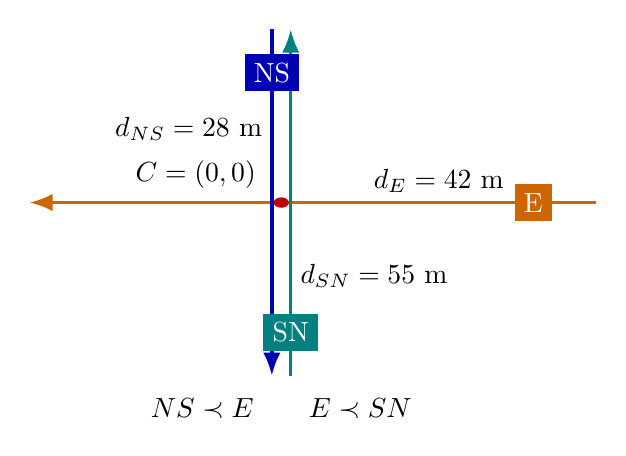
\begin{tikzpicture}[x=.8cm,y=.55cm,>=Latex]
\draw[->,very thick,orange!80!black](5,0)--(-4,0);
\draw[->,very thick,blue!70!black](-.15,4)--(-.15,-4);
\draw[->,very thick,teal](.15,-4)--(.15,4);
\node[fill=orange!80!black,text=white]at(4,0){E};
\node[fill=blue!70!black,text=white]at(-.15,3){NS};
\node[fill=teal,text=white]at(.15,-3){SN};
\fill[red!75!black](0,0)circle[radius=.12];
\node[above left,fill=white]at(-.25,.1){$C=(0,0)$};
\node[above]at(2.5,0){$d_E=42$ m};
\node[left]at(-.15,1.7){$d_{NS}=28$ m};
\node[right]at(.15,-1.7){$d_{SN}=55$ m};
\node[below]at(0,-4.3){$NS\prec E\qquad E\prec SN$};
\end{tikzpicture}\end{center}
\textbf{图 3：共用一个中心参考的最小耦合问题。}图为抽象示意，车道偏移及距离不按比例。取
\[
d_E=42,\qquad d_{NS}=28,\qquad d_{SN}=55\quad(\mathrm m).
\]
两组关系选择 $NS\prec E$、$E\prec SN$。设 $D_{\min}=12$ m：
\[
h_{NS,E}=42-28-12=2\unit{m},\qquad h_{E,SN}=55-42-12=1\unit{m}.
\]
三车速度均为 10 m/s 时初始高阶裕量也非负。同一 $d_E$ 同时进入两条约束；不再区分 $d_E^1,d_E^2$。共用参考点不意味着对没有交叉关系的 NS 与 SN 增加让行约束。


\page{多少车辆才能形成持续的多约束问题？}
设整圈长度为 $L$、车辆数为 $N$、单方向协调窗口为 $W$。均匀空间分布下平均间距为 $\Delta=L/N$，三个方向窗口的车辆总数期望为
\[
\bar n_{\mathrm{win}}=\frac{3WN}{L}.
\]
它是平均占有量，不足以单独判断双冲突；还要检查同一 E 是否同时遇到 NS、SN，以及两对距离差是否小于 $D_{\min}+h_{\mathrm{act}}=20$ m。
\begin{center}\small
\begin{tabular}{rrrrr}\toprule
$N$ & $\Delta$（m） & $\bar n_{\rm win}$ & 双窗口（\%） & 双距离触发（\%）\\\midrule
10 & 150.00 & 1.20 & 0.0 & 0.0 \\
12 & 125.00 & 1.44 & 46.6 & 46.6 \\
16 & 93.75 & 1.92 & 0.0 & 0.0 \\
18 & 83.33 & 2.16 & 69.9 & 69.9 \\
20 & 75.00 & 2.40 & 40.0 & 0.0 \\
22 & 68.18 & 2.64 & 64.0 & 0.0 \\
24 & 62.50 & 2.88 & 93.2 & 93.2 \\
26 & 57.69 & 3.12 & 100.0 & 0.0 \\
30 & 50.00 & 3.60 & 100.0 & 100.0 \\
36 & 41.67 & 4.32 & 100.0 & 100.0 \\
\bottomrule

\end{tabular}\end{center}
\textbf{计算方法：}固定 $L=1,500$ m、$W=60$ m，将均匀车列整体空间偏移扫过 $[0,\Delta)$，取 1,200 个中点。每个样本逐车检查两组关系，全部使用到中心的纵向距离；EW 的路线中心事件为 1.75 m，NS/SN 分别为 500/1000 m。2,400 点复核后主配置比例差小于 0.2 个百分点。没有运行车辆动力学或按时间预测碰撞。

\textbf{建议分工：}10 辆作为稀疏对照；18 辆约 69.9\% 的双触发需求作为中等负载；24 辆约 93.2\% 作为主优化场景；30/36 辆进一步引入同窗口多辆候选，检查排队与饱和。

26 辆虽常有双窗口共现，但本均匀分布下不同时满足两组 20 m 接近阈值；这说明数量不等于难度。数量是 3 的倍数时，三个等长通行段容易造成距离对齐，正好可以用来制造压力，而不再被直接排除出研究。

\textbf{重要：}均匀对齐样本常有 $h<0$，不能直接当作已经满足安全集合的初值。上表是未控制的几何需求分布。正式闭环使用第 \ref{sec:init} 节的非均匀可行初始化，保留均匀对齐组用于专门的初始不可行恢复研究。


\page{距离安全裕量与窗口尺度}
\subsection{空间阈值从车身尺寸出发，而不是时间换算}
设车长 $\ell=4.8$ m、车宽 $b=2.0$ m、每端裕量 $m=0.5$ m、南北车道中心横向偏移 $w/2=1.75$ m。合并为中心参考后，采用保守的统一纵向占用半长
\[
a_C=\ell/2+b/2+m+w/2=5.65\unit{m}.
\]
EW 的实际交叉区域相对中心偏移 $\pm1.75$ m，必须计入；对 NS/SN 也使用同样的上界，得到一个保守、统一的中心占用模型。若一对交叉车辆同时占用相应膨胀区域，则都满足 $d_i,d_j\in[-a_C,a_C]$，从而 $d_j-d_i\leq2a_C=11.3$ m。故保持有序差值至少 $D_{\min}=12$ m 可排除该简化模型的同时占用。

12 m 超出该界的余量只有 0.7 m，不应沿用旧双点模型的余量解释。实际车型包围盒、跟踪误差、定位偏差及偏航可能需要更大阈值；调整阈值后重算需求和 QP 初态。所有事件至少保持到相应前行车辆 $d<-a_C$ 并核验车身已清空。该几何说明依赖正交直行和固定路径，不是所有姿态的安全证明。

\subsection{两个阈值的分工}
\begin{itemize}
\item $D_{\min}=12$ m 是有序距离分离要求。
\item $h_{\mathrm{act}}=8$ m 是距离接近/优化需求标记：$|d_i-d_j|<20$ m。它用于统计与调节干预权重，不能作为任意删除硬安全约束的理由。
\item $W=60$ m 是候选车辆的空间范围；相关已承诺事件即使车头过点也继续保留到车尾清空。
\end{itemize}
\begin{center}\small
\begin{tabular}{rrrr}\toprule
$W$（m） & 双窗口（\%） & 双距离触发（\%） & 单车道至少两候选（\%）\\\midrule
40 & 61.2 & 61.2 & 0.0 \\
60 & 93.2 & 93.2 & 0.0 \\
80 & 100.0 & 100.0 & 30.8 \\
\bottomrule

\end{tabular}\end{center}
固定 1,500 m、24 辆，60 m 窗口能产生频繁双约束需求，且均匀车列每方向通常至多一辆候选；80 m 窗口增加同方向多车，但已超过最短直线段，需要曲线路径距离和更多约束。40 m 窗口适合作为提前量不足的对照，不是首选。

\textbf{保持约束的条件：}所有有效冲突候选都要检查高阶条件；不能只在 $h$ 很小时才发现相对速度已无法纠正。进入窗口或切换顺序时重新检查可行性，必要时使用更远的监测区与停车备份。


\page{控制结构：距离反馈与一致的通行顺序}
\begin{center}
\begin{tikzpicture}[node distance=5mm,>=Latex,box/.style={draw=Teal,fill=Teal!4,rounded corners,text width=12.2cm,minimum height=10mm,align=center,font=\small}]
\node[box](a){定位到有向路线：累计弧长、分支、到统一中心的有符号距离};
\node[box,below=of a](b){距离决策：近者优先 + 可行性检查 + 已承诺顺序保持};
\node[box,below=of b](c){名义速度/间距控制 + 联合距离高阶 CBF-QP};
\node[box,below=of c](d){纵向 PID 与横向 Pure Pursuit};
\node[box,below=of d](e){执行油门、制动、转向；反馈实际距离与速度};
\foreach \p/\q in {a/b,b/c,c/d,d/e}{\draw[->](\p)--(\q);}
\end{tikzpicture}
\end{center}
\subsection{名义控制不预设到达时间表}
令 $g_i$ 为沿同一有向闭环到前车的参考点间距。初版名义控制为
\[
u_i^{\nom}=k_v(v^*-v_i)+k_g(g_i-g^*)+k_r(v_{i+1}-v_i),
\]
其中 $v^*=10$ m/s、$g^*=L/N$，初始增益为 $k_v=0.5$ s$^{-1}$、$k_g=0.02$ s$^{-2}$、$k_r=0.3$ s$^{-1}$。不使用全局时间相位追踪项。

\textbf{均匀间距不是不可更改的硬目标。}24 辆在三个等长段上均匀分布会造成冲突距离对齐，故严格追求 $g_i=L/N$ 与无冲突恒速可能不相容。先用它作为软参考并观察与 barrier 的冲突；对照实验应减弱 $k_g$，或优化固定的非均匀目标 $g_i^*$，满足 $\sum g_i^*=L$ 与各距离约束。不能把由此产生的持续制动误称为已收敛。

\subsection{通行顺序规则}
对尚未承诺的车辆，用同一路口中心的纵向剩余距离较小者作为优先候选；距离接近时以进入范围顺序、ID 打破平局。随后必须检查 $h\geq0$、高阶初始条件与输入可行性。距离较近但明显更慢的车辆仍可能使该顺序不可行，应提前协调或停车，不能用“近者先行”替代可行性分析。

顺序按某次车辆通行事件记录，两组交叉关系联合检查，禁止形成循环等待。车尾清空前保持承诺，不因一帧测量波动反复翻转。速度只用于距离变化率、动力学与可行性检查，不用于计算 TTC 优先级。


\page{同样 24 辆车：一个可行的非均匀空间目标}
仅增加车辆数制造冲突还不够，也需要确认存在值得趋近的队形。对同一条 1,500 m 路线，构造 8 个三车小队，组间重复周期 187.5 m，组内车辆参考点间距 20 m：
\[
s_{k,j}=187.5k+20j,\qquad k=0,\ldots,7,\quad j=0,1,2.
\]
沿整圈的参考点间距按 $(20,20,147.5)$ m 重复，合计仍是 24 辆、1,500 m。采用 4.8 m 车长时，组内净车距为 15.2 m。
\begin{center}
\begin{tikzpicture}[x=.045cm,y=1cm,>=Latex]
\draw[->](-10,0)--(240,0);
\foreach \x/\lab in {0/1,20/2,40/3,187.5/4,207.5/5,227.5/6}{
\node[fill=Teal,text=white,minimum width=5mm,minimum height=4mm,font=\small]at(\x,0){\lab};}
\draw[<->](0,-.5)--(20,-.5) node[midway,below,font=\small]{20};
\draw[<->](20,-.5)--(40,-.5) node[midway,below,font=\small]{20};
\draw[<->](40,-.5)--(187.5,-.5) node[midway,below,font=\small]{147.5 m};
\node[above]at(20,.4){三车组 1};\node[above]at(207.5,.4){三车组 2};
\end{tikzpicture}
\end{center}
\subsection{完全用空间位移验证}
若每车以相同速度保持此队形，对于一组交叉关系的两个中心截面路线事件坐标 $s_e,s_f$，枚举不同车辆对并计算
\[
\delta_{ij}^{ef}=(s_f-s_j-s_e+s_i)\bmod L,\qquad
q_{ij}^{ef}=\min(\delta_{ij}^{ef},L-\delta_{ij}^{ef}).
\]
这是让整列车沿路线共同平移时，两次交叉事件之间的\textbf{空间位移差}，单位 m，没有除以速度。对 $EW/SN:(1.75,1000)$ 和 $EW/NS:(1.75,500)$ 分别枚举后得到
\[
q_{\min}^{EW/SN}=20.75\unit{m},\qquad q_{\min}^{EW/NS}=24.25\unit{m}.
\]
两者均高于 12 m 中心距离分离要求。因此，在理想等速、固定路径和车身假设下，\textbf{同样 24 辆存在满足距离分离的非均匀周期队形}。它比“降低到很少车辆”更适合研究车队重组与冲突优化。

\subsection{如何用于实验，而不把目标当结果}
\begin{itemize}
\item 使用 \texttt{cluster\_target.csv} 做队形保持实验，检验 PID、路线与距离过滤器是否能保持该状态。
\item 使用非均匀可行扰动初态做恢复实验；名义间距参考可取按车辆循环顺序分配的 $(20,20,147.5)$，避免强行回到不利的均匀间距。
\item 初始扰动到此目标是否始终存在安全可行路径、能否由所选局部反馈收敛，仍需分析与 CARLA 实验。不能仅由目标可行推断过程可行。
\end{itemize}
这个构造不是数值搜索得到的最优队形；之后可优化组内间距、组数及叶瓣长度比例，以比较通行平顺性、制动和恢复时间。

\page{从距离 barrier 推导加速度：必须使用二阶关系}
对已确定 $i$ 先、$j$ 后的冲突事件，定义
\[
h=d_j-d_i-D_{\min},\qquad \dot d_i=-v_i,\qquad \dot v_i=u_i.
\]
于是
\[
\dot h=v_i-v_j,\qquad\ddot h=u_i-u_j.
\]
\textbf{关键区别：}距离函数对加速度的相对阶为 2，$\dot h+\kappa h\geq0$ 中没有加速度。因此不能照搬上一版时间 barrier 的一阶公式，也不能只将秒换成米。

\subsection{候选高阶 CBF 条件}
令 $k_1,k_2>0$，定义
\[
\psi_1=\dot h+k_1h,\qquad\dot\psi_1+k_2\psi_1\geq0.
\]
展开为线性加速度约束：
\begin{equation}\boxed{u_i-u_j+(k_1+k_2)(v_i-v_j)+k_1k_2h\geq0.}\end{equation}
高阶 CBF 的一般形式见\cite{xiao}。需同时满足初始 $h\geq0$ 和 $\psi_1\geq0$，并在模型有效、顺序固定和输入可行期间持续执行；不能从任意相同距离初态直接宣称安全。初取 $k_1=k_2=0.5$ s$^{-1}$，后续测试 0.2、0.5、1.0 的组合。

\subsection{两组冲突共同限制同一辆 E}
在第 5 节的初态，三车速度相同，得到
\[
u_{NS}-u_E+0.5\geq0,\qquad u_E-u_{SN}+0.25\geq0.
\]
举例假设当前名义加速度为 $(u_E^{\nom},u_{NS}^{\nom},u_{SN}^{\nom})=(1,0,2)$ m/s$^2$。该向量用于演示求解，不声称由第 \ref{sec:init} 节的完整车队名义控制自动算出。联合最小化 $\tfrac12\|\mathbf u-\mathbf u^{\nom}\|^2$，约束上式及 $-3\leq u\leq2$，得到
\[
\boxed{(u_E^*,u_{NS}^*,u_{SN}^*)=(1.083333,\ 0.583333,\ 1.333333)\unit{m/s^2}.}
\]
两条约束均取等号，非负 KKT 乘子约 $(0.583333,0.666667)$。E 的一次加速既受前方 NS 限制，又影响后行 SN；这正是联合优化相对于独立修正相加的意义。

完整车队 QP 加入所有有效距离冲突、同路线跟车和输入约束；jerk 只作软惩罚。同路线跟车可用 $h_f=g_i-\ell-d_0$ 的二阶条件，$d_0=5$ m 起步，并结合实际制动可行域验证。执行器误差 $|e_i|\leq\bar e_i$ 时，上式右侧收紧为 $\bar e_i+\bar e_j$；未标定上界不能默认为零。


\page{PID 与横向控制：把加速度变成实际车辆动作}
\subsection{纵向接口与速度参考}
QP 输出单位是 m/s$^2$，CARLA 油门和制动输入是归一化执行器量，两者不能直接等同。每个 0.05 s 周期由当前测量速度构造一小步目标
\[
v_{\mathrm{ref},k+1}=\operatorname{clip}(v_k+u_k^*\Delta t,0,v_{\max}).
\]
低层可保持这个目标一个周期；若改为累计参考积分，应加入饱和时的参考回退，防止目标漂移。由于一小步速度误差较小，单靠速度 PID 未必能跟踪所需加速度，应标定油门/制动前馈 $q_{ff}(v,u^*)$。
\[
e_k=v_{\mathrm{ref},k+1}-v_k,\quad
q_k=q_{ff}+K_pe_k+K_i I_k+K_d\dot e_{f,k},\quad -1\leq q_k\leq1.
\]
令 throttle$=\max(q_k,0)$，brake$=\max(-q_k,0)$；两者不同时为正。输出饱和且积分会继续推动饱和时暂停积分，$I$ 初始限幅为 $\pm3$ m。微分滤波时间常数取 0.15 s。

\begin{center}\small
\begin{tabular}{llll}\toprule
参数 & 初值 & 首轮范围 & 单位\\\midrule
$K_p$ & 0.25 & 0.10--0.50 & s/m\\
$K_i$ & 0.03 & 0--0.08 & 1/m\\
$K_d$ & 0.02 & 0--0.05 & s$^2$/m\\\bottomrule
\end{tabular}\end{center}
上述是无量纲油门/制动输出对应的增益单位，不是 CARLA 内置控制器参数的通用默认值。先在直线上做 5、8、10、12 m/s 定速与 $-2,-1,0,1,2$ m/s$^2$ 的安全加速度跟踪试验，拟合前馈，再依次调 P、I、D。记录响应延迟、饱和、稳态误差和实际加速度误差。

\subsection{横向 Pure Pursuit 与曲率约束}
横向跟踪选 Pure Pursuit\cite{coulter}。用路线方向选择前视点，$L_d=5+0.5v$ m；在车辆坐标系中记目标夹角为 $\alpha$，轴距为 $l_w$，则
\[
\delta=\arctan\!\left(\frac{2l_w\sin\alpha}{L_d}\right).
\]
轴距、转角上限和 steering 归一化关系由实际车型标定；不要把弧度直接传给 $[-1,1]$ 的 steer。中央路口不得由最近 waypoint 的任意分支选择来决定路线。先验证单车不少于三圈，无逆行、切角、跳支，再接入多车控制。

\page{定位：世界坐标、路线弧长与圈数}
\subsection{第一阶段用真值，避免无关复杂度}
CARLA 提供 actor 的位置、速度及加速度接口\cite{carla_api}。首先读取世界位置 $(x,y,z)$，投影到指定路线。控制使用沿路线切向的速度 $v=\mathbf v\cdot\mathbf t(s)$；不能在倒车或错误分支情况下仍使用速度向量模长掩盖方向错误。

路线几何以东、北为正，UE/CARLA 使用不同的坐标约定。导入时显式保存变换，例如选取平移原点并采用 $x_C=x_0+x$、$y_C=y_0-y$、$z_C=z_0$；朝向同步变换。该关系需用东、西、南、北各一个检查点验证，不能只看渲染图是否“像”。

\subsection{交叉点处不能只找最近中心线}
同一 $(x,y)$ 在本路线可对应不同弧长。每车保存上一段 primitive ID、累计弧长 $S$、分支和已承诺事件；只在前后可达弧长窗口内投影，并用车头方向作一致性检查。
\begin{enumerate}
\item 用 $S_{k-1}+v_{k-1}\Delta t$ 预测当前位置。
\item 在预测附近及已知后继段中搜索投影，初始窗口可取 $\pm10$ m。
\item 选择位置误差小且方向一致的解；无合法解则报告定位/路线故障，不跳到另一条交叉车道。
\item 把模 $L$ 的 $s$ 展开到距预测最近的圈次，得到 $S=s+nL$。
\item 计算下一个尚未完成的\emph{事件实例}距离，不能简单选最近物理冲突点。
\end{enumerate}

OpenDRIVE/CARLA waypoint 的 \texttt{road\_id}、\texttt{lane\_id}、\texttt{s} 用于路网匹配\cite{carla_map}。其中 \texttt{s} 是道路参考线坐标，不是整圈累计弧长；某些车道的行驶方向与参考线递增方向相反。应将 actor 原点转换为车辆几何中心，并单独维护 road/lane 到路线段的映射，导入后再生成实际中心线采样。

\subsection{后续才加入估计误差}
CARLA 的 GNSS 依赖 OpenDRIVE 地理参考，IMU 则提供惯性测量\cite{carla_sensors}。基线无需先估计经纬度；若研究定位影响，先对路线投影位置加入有记录的噪声和延迟，再扩展 GNSS/IMU 融合。

噪声测试取位置标准差 0.1/0.3/0.5 m、延迟 0.05/0.1/0.2 s，保存同一时刻的真值与估计值。控制只使用估计值，独立安全评估使用真值，避免把真值泄漏进被测试的估计控制链。

\page{从参数化中心线到 OpenDRIVE 地图}
\subsection{格式与制作路径}
\begin{center}\small
\begin{tabular}{P{2.7cm}P{5cm}P{5.8cm}}\toprule
格式 & 本项目角色 & 是否能直接构成 CARLA 路网\\\midrule
SVG / TikZ & 地图图示、尺寸和方向审阅 & 否；缺道路、车道和连接语义\\
JSON / CSV & 参数、路线采样、冲突事件 & 否；作为生成器与验证器输入\\
OpenDRIVE .xodr & 道路参考线、车道、junction 连接 & 可通过 standalone 模式生成道路\cite{carla_odr}\\
网格与场景资产 & 地形、建筑、材质、装饰 & 单独网格不替代可导航车道拓扑\\\bottomrule
\end{tabular}\end{center}

\subsection{建议的建图步骤}
\begin{enumerate}
\item 以本文直线/圆弧作为 G1 种子，加入缓和段，重新求连接与段长；保留中央两车道间距。
\item 把三条中央通行方向和各外侧叶瓣划分成道路段。为每段定义参考线、车道宽度、行驶方向和 predecessor/successor。
\item 中央建立一个 junction，定义 EW、NS、SN 三个直行 movement 的连接道路及 lane links。不能只让三条网格在空间上重叠，也不能把不同方向错误链接为可转弯分支。
\item 外侧每个出口只连接唯一后继入口。用有向图检查所有有效车道属于一个目标循环，没有死路、错误回路或额外合流。
\item 从导出的地图重新采样，计算实际路径长度、曲率、车道边界和冲突区域；重新生成统一中心截面事件并进行距离冲突扫描。
\item 在 CARLA standalone 中先空地图检查，再一辆车验证；通过后才考虑路面材质、景观和 Unreal 完整资产流程。
\end{enumerate}

\subsection{车道中心线不等于道路参考线}
本文几何描述的是车辆行驶中心线。若用一条道路承载两个反向车道，道路参考线应位于两车道之间；车道中心线还包含横向偏置。若直接把本文坐标当参考线又追加半车道宽偏置，会改变冲突点位置和半径，导致距离统计失效。

OpenDRIVE 可使用 line/arc/spiral 等几何描述。程序化生成适合可重复参数扫描；RoadRunner 等编辑器可辅助检查，但不是本项目必须采购的依赖。\textbf{当前没有 .xodr 文件，也没有声称完成 CARLA junction 验收。}

\page{CARLA 环境：版本、硬件与运行方式}
\subsection{可复现的目标环境}
本报告选择有固定发布包的 CARLA 0.9.15\cite{carla_release}，避免用“最新版本”作为可变依赖。Ubuntu 22.04 x86-64 是实验主机目标；应先运行发布包自带示例确认显卡驱动与系统兼容。旧版安装文档中的 Debian 仓库支持范围不同，本项目优先采用发布包，不照抄旧 apt 仓库安装命令。

官方 0.9.15 快速开始文档给出 Windows/Linux 平台、至少 6 GB 显存（推荐 8 GB）、约 20 GB 安装空间，以及默认 2000/2001 端口\cite{carla_start}。本文额外建议预留 32 GB 内存、12 GB 或以上独立显存和 50 GB 可用磁盘，作为多车、日志与观测余量；这不是官方硬性最低要求。

当前 Mac 可完成 LaTeX、离线设计及结果分析。服务器放在 Linux x86-64 主机，本地或远程运行 Python 控制器均可；为了降低抖动，首轮把控制器与服务器放在同一主机。图像仅保留一个观测相机或 spectator，不给每车挂多路高分辨率传感器。

\subsection{安装与版本核对步骤（待执行）}
\begin{enumerate}
\item 下载固定的 0.9.15 Linux 发布包，记录下载地址、压缩包校验和、GPU/驱动信息。
\item 建立独立 Python 环境，使用与 Python ABI 和平台匹配的 CARLA 0.9.15 wheel；优先从发布包选择匹配文件。无匹配 wheel 时调整 Python 版本，不能混装其他版本客户端。
\item 启动 \texttt{CarlaUE4.sh}，连接后记录 \texttt{get\_client\_version()} 与 \texttt{get\_server\_version()}，不一致则停止实验。
\item 验证普通地图单车示例，再使用未来制作的自定义地图进行 standalone 导入。
\end{enumerate}

\subsection{同步与物理步长}
仿真使用同步模式，每帧固定 $\Delta t=0.05$ s，控制同频更新。物理子步上限 0.01 s、最多 10 步，满足
\[
\Delta t\leq\texttt{max\_substep\_delta\_time}\times\texttt{max\_substeps}.
\]
只允许一个控制客户端调用 \texttt{world.tick()}；观察端不得再次推进仿真。传感器消息与状态按 frame 对齐，不能混用墙上时间与仿真时间。固定时间步的配置依据官方同步文档\cite{carla_sync}。

\page{加载与生成车辆：未来接口示例}
以下片段用于说明未来调用流程，\textbf{不是本次已运行的地图导入脚本}。变量 \texttt{xodr\_path} 必须指向已制作并检查过的地图，\texttt{validated\_spawn} 必须来自该地图的目标路线。
\begin{lstlisting}[language=Python]
from pathlib import Path
import carla

client = carla.Client("127.0.0.1", 2000)
client.set_timeout(60.0)
assert client.get_client_version() == client.get_server_version()
text = Path(xodr_path).read_text(encoding="utf-8")
params = carla.OpendriveGenerationParameters(
    vertex_distance=1.0, max_road_length=50.0,
    wall_height=1.0, additional_width=0.6,
    smooth_junctions=True, enable_mesh_visibility=True)
world = client.generate_opendrive_world(text, params)
original = world.get_settings()
settings = world.get_settings()
settings.synchronous_mode = True
settings.fixed_delta_seconds = 0.05
settings.substepping = True
settings.max_substep_delta_time = 0.01
settings.max_substeps = 10
world.apply_settings(settings)
actors = []
try:
    bp = world.get_blueprint_library().find("vehicle.tesla.model3")
    for transform in validated_spawn:
        actor = world.try_spawn_actor(bp, transform)
        if actor is None:
            raise RuntimeError("spawn failed; do not reduce fleet silently")
        actors.append(actor)
        actor.set_autopilot(False)
    frame = world.tick()
    snapshot = world.get_snapshot()
    # Next: initialize route/event states, then run one controller tick.
finally:
    for actor in actors:
        actor.destroy()
    world.apply_settings(original)
\end{lstlisting}
standalone 接口接收 OpenDRIVE 的\textbf{内容字符串}，不是文件路径。junction 平滑与额外宽度可能改变可见网格，需检查最终网格和逻辑车道的一致性\cite{carla_odr}。上面的清理恢复的是加载后世界的时间设置，不会恢复加载前的旧地图。

\textbf{生成策略：}依路线坐标插值姿态，结合路面高度设置小的生成高度偏移；所有车辆逐一检查可生成性。固定 $N$ 不能因生成失败而悄悄减小。初始非零速度只可作为明确记录的初始化条件；控制运行期间不通过强制速度或传送车辆替代油门/制动。

\page{在线循环、顺序状态机与日志}
\subsection{每帧执行一次完整闭环}
\begin{enumerate}
\item 获取同一 frame 的位置、速度、加速度；更新路线投影、圈数与分支。
\item 更新冲突区域进入/占用/清空状态，保持已承诺事件顺序。
\item 对未承诺候选事件按距离排序、检查高阶条件与顺序可行性；同一路口两冲突联合处理。
\item 计算名义加速度，形成有序冲突、跟车与输入约束并求解 QP。
\item 有解则转为 PID 参考及转向命令；无解则记录并进入预先验证的备份逻辑。
\item 批量发送本帧命令，再调用一次 tick；在下一帧记录实际响应。
\end{enumerate}
\subsection{控制权限必须清楚}
研究车辆使用自定义控制并关闭 autopilot，不由 Traffic Manager 同时控制。地图中的信号灯、让行标记应检查并明确设定；若冻结信号灯，保存并在退出时恢复设置。物理碰撞仍保留，不能通过关闭碰撞让距离控制看起来成功。

不能把 CARLA Traffic Manager 的自动避让、传送、车辆销毁或信号遵守算成 barrier 的效果。碰撞事件、失踪车辆、数量变化、QP 无解与路线跳支都作为失败记录，不能从样本中剔除。

\begin{center}\small
\begin{tabular}{P{3.1cm}P{10.3cm}}\toprule
日志组 & 至少保存的字段\\\midrule
实验标识 & seed、版本、地图与配置哈希、车型、生成成功数、控制方法\\
车辆状态 & frame、仿真时间、ID、$x,y,z$、yaw、$S,s,$圈数、branch、速度、实际加速度\\
控制状态 & $u^{\nom},u^*$、PID 参考、throttle、brake、steer、饱和状态\\
事件约束 & event ID、中心 ID、交叉关系、前后顺序、有符号距离、$h,\psi_1$、占用进入与清空状态\\
求解与安全 & QP 状态/耗时、最小约束余量、碰撞、最小车身距离、定位跳变\\\bottomrule
\end{tabular}\end{center}
车辆加速度向路线切向投影后再用于纵向误差统计；弯道上直接用加速度向量模长会把向心加速度误当成纵向加速。jerk 采用固定步长差分并保存滤波方法。

\textbf{停止边界示例：}10 m/s、可用制动 3 m/s$^2$、总延迟 0.15 s 时，理想停止距离约 $10^2/(2\cdot3)+10\cdot0.15=18.17$ m，再加模型与定位余量。60 m 是初始协调窗口，不是无条件安全距离；实际制动能力必须标定。

\page{24 车可行初始化与实验矩阵}
\label{sec:init}
\subsection{不要把均匀对齐的压力分布直接当安全初值}
在 1,500 m 环上先放置 $s_i=(i+0.5)L/24$。再将最接近三处目标的车辆分别置于
\[
s_E=1500+1.75-42=1459.75,\quad s_{NS}=500-28=472,\quad s_{SN}=1000-55=945\unit{m}.
\]
其余车辆保持原位置。生成文件 \texttt{initial\_positions.csv} 含全部 24 辆的固定初态。全车速度设 10 m/s，沿路线最小参考点间距为 38.75 m；当前三个接近窗口各有一辆，两个有序距离裕量分别为 2 m 和 1 m，$\psi_1$ 分别为 1 与 0.5 m/s。

这是初始距离条件与局部约束的检查，不是未来一圈始终可行的证明。车辆应在 CARLA 中确认车身不重叠、道路姿态正确、跟车与全车 QP 可行后启动。生成失败不能减少 $N$，也不能借传送车辆“恢复”。
\begin{center}\small
\begin{tabular}{P{2.3cm}P{5.6cm}P{5.6cm}}\toprule
阶段 & 配置 & 用途\\\midrule
S0 & 单车，完整路线三圈 & 定位、转向与 PID 标定\\
S1 & 图 3 的三车局部相遇 & 验证同一 E 的两条距离约束\\
S2 & 18 辆，安全筛选初态 & 中负载，观察重复交叉协调\\
S3 & 24 辆，所给非均匀初态 & 主优化实验；测试速度/位置扰动恢复\\
S4 & 30、36 辆 & 多候选、排队、制动饱和与无解边界\\
S5 & $W=40/60/80$ m & 提前量与求解规模敏感性\\\bottomrule
\end{tabular}\end{center}
采用种子 11、22、33、44、55；位置扰动 2/5 m、速度扰动 0.5/1 m/s 均需重新检查 $h,\psi_1$ 与 QP 可行性，记录拒绝率。最多运行 15 圈，连续三圈观察稳态。

\textbf{稳态指标：}无碰撞、无占用重叠、无 QP 无解、固定车数；有效约束 $h\geq0,\psi_1\geq0$；速度 RMS/最大误差不超过 0.3/0.8 m/s；低于 0.5 m/s 持续 1 s 计停车；brake$>0.01$ 帧占比低于 1\%；纵向加速度 RMS 不超过 0.2 m/s$^2$，jerk 95 分位不超过 1 m/s$^3$。这些是待测试标准。

对比：纯名义跟驰、独立两两距离启发式、联合距离 HOCBF-QP。另比较均匀软间距与非均匀间距参考。均匀距离重合组作为初始不可行恢复专题，不与初始安全组混算收敛成功率。完全零制动需单独报告，不能用“低制动”替代。


\page{已完成的距离版检查与下一步}
\begin{center}\small
\begin{tabular}{P{4cm}P{9.3cm}}\toprule
检查 & 本次结果\\\midrule
几何 & 1,500 m 闭合 G1 中心线；仅中央两处预期交叉；最小半径 51.803 m\\
道路带 & 0.5/0.25 m 采样，中央 $16\times16$ m 交叉区外无额外非局部重叠\\
车数扫描 & 24 辆、60 m 窗口：双距离触发需求约 93.2\%；10 辆对照为 0\\
空间扫描精度 & 1,200/2,400 偏移样本对主配置结果差小于 0.2 个百分点\\
初始化 & 24 辆固定；局部 $h=(2,1)$ m，$\psi_1=(1,0.5)$ m/s\\
加速度推演 & 三车距离 HOCBF-QP 候选解通过约束与 KKT 检查\\
短时回放 & 该三车恒加速度执行 0.05 s，每 1 ms 检查距离裕量非负\\\bottomrule
\end{tabular}\end{center}
空间需求率不是仿真安全率；短时回放也不是整个车队动态仿真。道路带验证排除弧长相距小于 10 m 的连续局部邻段，以及预期中央交叉区，容差 0.005 m。曲率跳变、路肩、车身姿态和未来生成网格仍需另行验证。

\subsection{需要实现的工程链}
\begin{enumerate}
\item 细化缓和段并制作 OpenDRIVE；重新计算各分支到统一中心截面的路径距离。
\item 完成单车路线、签名距离与跨圈事件定位，校准 PID 和实际加速度误差。
\item 加入距离排序、承诺/车尾释放状态机、距离高阶约束和 QP 无解备份。
\item 先验证三车双约束，再运行 18/24/30 辆；比较求解活跃约束数、干预量、制动与恢复。
\item 若均匀间距目标导致持续对抗，优化空间间距分布或三个叶瓣长度比例；不恢复使用 TTC 作为判断准则。
\end{enumerate}

\textbf{什么才算展示了优化价值？}同一车辆确实同时面对两条有效约束；联合方法相对独立修正在碰撞、距离违规、无解率和舒适性上有可重复改善。仅“地图有交叉”或“车开了几圈没撞”不足以支撑该结论。

\textbf{关于稳定通行：}保持固定车辆数、让行顺序与安全距离是设计要求；从哪些初值可以恢复、是否需要非均匀车距、能否最终不刹车是实验与理论要回答的问题。24 辆不是预先保证能匀速通过的答案，而是能持续暴露耦合距离冲突的研究配置。


\page{文件组织、复算步骤与参考资料}
\begin{center}\small
\begin{tabular}{P{5.1cm}P{8.1cm}}\toprule
文件/目录 & 用途\\\midrule
\texttt{report\_zh.tex / .pdf} & 本报告源文件与最终 PDF\\
\texttt{references.bib} & 官方文档与控制理论来源\\
\texttt{config/*.json} & 地图、控制、实验参数；未标定项明确为 null 或设计初值\\
\texttt{scripts/analyze\_design.py} & 仅 Python 标准库的几何/距离冲突复算器\\
\texttt{figures/*.svg, *.tex} & 由实际采样生成的矢量地图、中央放大图和三车距离场景图\\
\texttt{results/*.csv, *.json} & 路线样本、24 车初态、距离需求扫描及几何结果\\
\texttt{results/*.tex} & 自动生成的报告数值与表格，避免手工转抄\\\bottomrule
\end{tabular}\end{center}
\subsection{当前可执行的命令}
从项目根目录运行：
\begin{lstlisting}[language=bash]
python3 'barrier 2vs1/scripts/analyze_design.py'
cd 'barrier 2vs1'
latexmk -xelatex -interaction=nonstopmode -halt-on-error report_zh.tex
\end{lstlisting}
Python 脚本无需 CARLA 或第三方包。编译 PDF 需要 XeLaTeX、ctex、TikZ 和 BibTeX；编译器生成的中间文件可放在独立临时构建目录。

修改地图参数后重新执行分析与编译，检查事件坐标、最小半径、道路带重叠和距离需求结果。脚本中的断言用于识别失效设计，不应为“让脚本通过”而删除。配置控制参数的变化不会自动变成 CARLA 实验结果。

\subsection{资料使用说明}
本报告的几何构造、参数推荐和距离扫描为本项目的设计与计算。CARLA 文档仅用于说明接口与平台能力；CBF 与 Pure Pursuit 文献提供方法背景。推荐参数均需实车模型标定，参考资料不构成该地图的安全或稳定性证明。

\clearpage
\small
\bibliographystyle{unsrt}
\bibliography{references}
\end{document}
